\documentclass[11pt]{article}

% -----------------------------------------------------------------------------
% Generic, venue-neutral manuscript skeleton.
% Replace the document class and formatting only after selecting a target venue.
% The file is intentionally standalone and should compile without external assets.
% -----------------------------------------------------------------------------

\usepackage[T1]{fontenc}
\usepackage[utf8]{inputenc}
\usepackage[a4paper,margin=1in]{geometry}
\usepackage{amsmath,amssymb}
\usepackage{booktabs}
\usepackage{array}
\usepackage{graphicx}
\usepackage{xcolor}
\usepackage{enumitem}
\usepackage{caption}
\usepackage{subcaption}
\usepackage{hyperref}
\usepackage{tikz}
\usetikzlibrary{arrows.meta,positioning,shapes.geometric,calc,decorations.pathreplacing,patterns}

\hypersetup{
  colorlinks=true,
  linkcolor=blue,
  citecolor=blue,
  urlcolor=blue
}

\newcommand{\placeholder}[1]{\textcolor{gray}{\emph{[#1]}}}
\newcommand{\methodname}{Selective Automation Framework}
\newcommand{\datasetname}{PCAOB Inspection-Finding Dataset}
\definecolor{figNavy}{HTML}{173B63}
\definecolor{figBlue}{HTML}{2E6F9E}
\definecolor{figPale}{HTML}{EAF3FA}
\definecolor{figPaler}{HTML}{F6FAFD}
\definecolor{figSlate}{HTML}{64748B}
\definecolor{figTeal}{HTML}{00796B}
\definecolor{figTealPale}{HTML}{E5F4F1}
\definecolor{figAmber}{HTML}{B26A00}
\definecolor{figAmberPale}{HTML}{FFF3D6}

\title{Calibrated Selective Classification of PCAOB Inspection Findings\\
with a Domain-Adapted Transformer}

\author{
  Author Name\\
  \small Affiliation\\
  \small \texttt{email@example.com}
}

\date{\today}

\begin{document}

\maketitle

\begin{abstract}
Public Company Accounting Oversight Board (PCAOB) inspection findings provide
machine-readable but heterogeneous narratives of audit deficiencies. Automating
their organization is useful for regulatory research, yet forcing a classifier
to label every finding can conceal uncertainty and taxonomy ambiguity. We study
selective automation of a researcher-defined 12-class audit-area taxonomy using
6,607 findings from 650 inspection reports. Reports, rather than individual
findings, are the partition unit, and near-duplicate controls are applied before
comparing a TF--IDF classifier, a frozen general-purpose sentence encoder, and an
end-to-end fine-tuned SEC-BERT model. SEC-BERT achieved the strongest
retrospective test point estimates (0.9337 accuracy and 0.9021 macro-F1), although
its 2.13-percentage-point accuracy advantage over TF--IDF had a report-cluster
95\% interval of $[-0.89,5.26]$ points. Temperature scaling reduced calibration
error. In a paired lexical-cue sensitivity analysis, the frozen canonical
SEC-BERT fell from 0.9021 to 0.2787 macro-F1 when explicit audit-area phrases
and standards references were masked without retraining; masked-input training
recovered macro-F1 to 0.5332. A simple top-two probability margin ranked label disagreements at
least as effectively as a learned risk router. Thresholds fixed on an independent
calibration set yielded two operating points: the high-coverage policy
automatically accepted 96.40\% of the 890-case test with 95.22\% accepted-set
agreement, while the conservative policy accepted 92.92\% with 96.61\%
agreement and captured 52.54\% of disagreements in the verification queue. The
results support calibrated,
risk-aware selective classification for retrospective PCAOB text organization;
they do not establish end-to-end human--machine accuracy or prospective temporal
robustness.
\end{abstract}

\noindent\textbf{Keywords:}
PCAOB inspection findings; selective classification; domain-adapted transformers;
uncertainty estimation; probability calibration; audit analytics

% Vector workflow figure; all text and geometry remain editable in LaTeX.
\begin{figure}[t]
  \centering
  \resizebox{\textwidth}{!}{%
  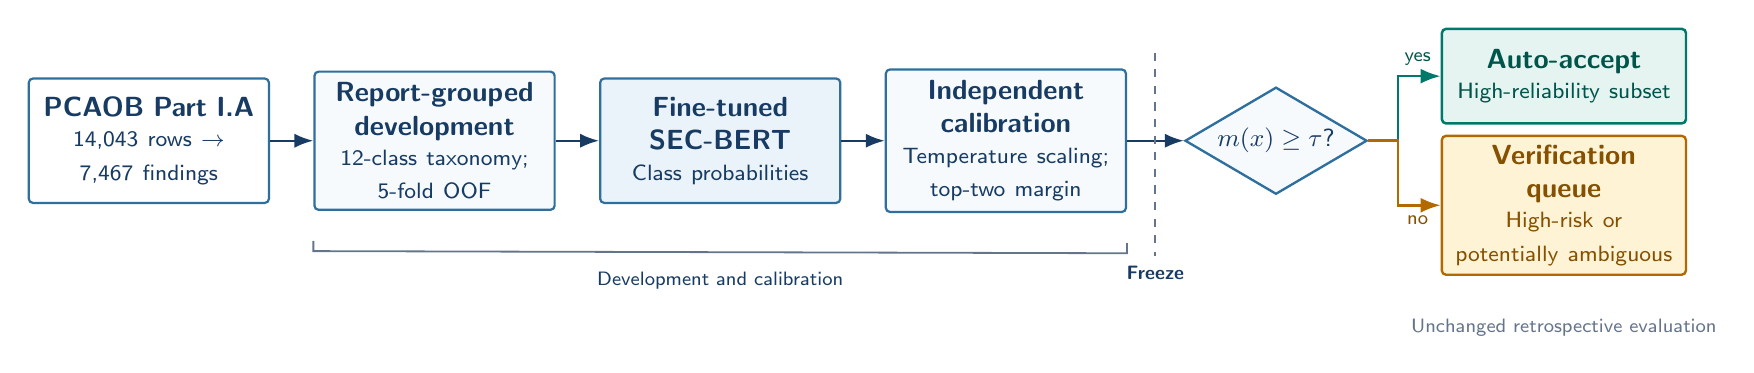
\begin{tikzpicture}[
    font=\sffamily,
    >=Latex,
    text=figNavy,
    flow/.style={-Latex, draw=figNavy, line width=0.85pt},
    acceptflow/.style={-Latex, draw=figTeal, line width=0.95pt},
    referflow/.style={-Latex, draw=figAmber, line width=0.95pt},
    stage/.style={
      rectangle, rounded corners=1.5pt, draw=figBlue, line width=0.8pt,
      fill=white, minimum width=3.05cm, minimum height=1.58cm,
      text width=2.72cm, align=center, inner sep=4pt
    },
    decision/.style={
      diamond, aspect=1.7, draw=figBlue, line width=0.85pt,
      fill=figPaler, minimum width=2.05cm, minimum height=1.35cm,
      align=center, inner sep=1.5pt
    },
    accepted/.style={
      rectangle, rounded corners=1.5pt, draw=figTeal,
      line width=0.9pt, fill=figTealPale, minimum width=3.10cm,
      minimum height=1.20cm, text width=2.78cm, align=center,
      text=figTeal!70!black
    },
    referred/.style={
      rectangle, rounded corners=1.5pt, draw=figAmber,
      line width=0.85pt, fill=figAmberPale, minimum width=3.10cm,
      minimum height=1.20cm, text width=2.78cm, align=center,
      text=figAmber!75!black
    }
  ]
    \node[stage] (source) {
      \textbf{PCAOB Part I.A}\\[-1pt]
      \footnotesize 14,043 rows $\rightarrow$ 7,467 findings};
    \node[stage, fill=figPaler, right=0.55cm of source] (development) {
      \textbf{Report-grouped development}\\[-1pt]
      \footnotesize 12-class taxonomy; 5-fold OOF};
    \node[stage, fill=figPale, right=0.55cm of development] (model) {
      \textbf{Fine-tuned SEC-BERT}\\[-1pt]
      \footnotesize Class probabilities};
    \node[stage, fill=figPaler, right=0.55cm of model] (calibration) {
      \textbf{Independent calibration}\\[-1pt]
      \footnotesize Temperature scaling; top-two margin};
    \node[decision, right=0.72cm of calibration] (decision) {
      \small $m(x)\geq\tau$?};

    \node[accepted, right=0.92cm of decision, yshift=0.82cm] (accept) {
      \textbf{Auto-accept}\\[-1pt]
      \footnotesize High-reliability subset};
    \node[referred, right=0.92cm of decision, yshift=-0.82cm] (refer) {
      \textbf{Verification queue}\\[-1pt]
      \footnotesize High-risk or potentially ambiguous};
    \draw[flow] (source) -- (development);
    \draw[flow] (development) -- (model);
    \draw[flow] (model) -- (calibration);
    \draw[flow] (calibration) -- (decision);
    \draw[acceptflow] (decision.east) -- ++(0.38,0) |- node[pos=0.73, above,
      font=\sffamily\scriptsize, text=figTeal!70!black] {yes} (accept.west);
    \draw[referflow] (decision.east) -- ++(0.38,0) |- node[pos=0.73, below,
      font=\sffamily\scriptsize, text=figAmber!75!black] {no} (refer.west);
    \coordinate (freezeTop) at ($(calibration.east)!0.50!(decision.west)+(0,1.12)$);
    \coordinate (freezeBottom) at ($(calibration.east)!0.50!(decision.west)+(0,-1.47)$);
    \draw[dashed, draw=figSlate, line width=0.7pt] (freezeTop) -- (freezeBottom);
    \node[below, font=\sffamily\scriptsize\bfseries] at (freezeBottom) {Freeze};

    \coordinate (bracketLeft) at ($(development.south west)+(0,-0.38)$);
    \coordinate (bracketRight) at ($(calibration.south east)+(0,-0.38)$);
    \draw[draw=figSlate, line width=0.65pt]
      (bracketLeft) -- ++(0,-0.13) -- ($(bracketRight)+(0,-0.13)$) -- (bracketRight);
    \node[below=0.13cm, font=\sffamily\scriptsize] at
      ($(bracketLeft)!0.5!(bracketRight)+(0,-0.13)$) {Development and calibration};
    \node[below=0.42cm of refer, font=\sffamily\scriptsize, text=figSlate]
      {Unchanged retrospective evaluation};
  \end{tikzpicture}%
  }
  \caption{Overview of the selective-automation framework. The solid path is
  developed using report-grouped out-of-fold predictions, calibrated on an
  independent split, and frozen before retrospective evaluation. Low-margin
  predictions enter a verification queue rather than receiving an automatic
  replacement label.}
  \label{fig:graphical-abstract}
\end{figure}

% =============================================================================
\section{Introduction}
\label{sec:introduction}
% =============================================================================

\subsection{Background and Motivation}

The Public Company Accounting Oversight Board (PCAOB) conducts inspections to
assess registered audit firms' compliance with applicable laws, rules, and
professional standards. Part~I.A of a public inspection report describes
deficiencies that the PCAOB considered sufficiently significant that the firm
had not obtained enough appropriate audit evidence to support the relevant audit
opinion. Since 2025, the PCAOB has distributed these findings in downloadable
machine-readable files containing the full deficiency descriptions, audit areas,
affected audits, cited standards, and related attributes
\cite{pcaob2025datasets}. The release makes systematic analysis more feasible,
but it does not remove the need to organize heterogeneous narrative text.
Prior accounting research has shown that coded types of PCAOB deficiencies can
support substantive analysis of later financial-reporting outcomes, while also
demonstrating the labor and judgment involved in constructing such categories
\cite{constance2025pcaob}.

The audit-area field contains fine-grained and historically variable expressions,
whereas a single finding may describe several accounts, transactions, controls,
and audit procedures. Manual normalization is costly and difficult to reproduce
at scale. Text classifiers can accelerate this work, and domain-adapted encoders
can exploit the specialized language of regulatory filings. Yet inspection
findings do not present a uniform level of classification difficulty. Some state
an account or transaction explicitly; others depend on an earlier report passage,
mix several audit areas, or describe only the mechanism of the audit deficiency.

This variation creates a practical tension for automatic classification.
Treating every case as straightforward maximizes automation
but conceals the errors made on ambiguous cases. Treating every case as difficult
avoids automatic error at the cost of eliminating the intended efficiency gain.
A useful system therefore requires a case-specific decision between automatic
acceptance and abstention. The decision cannot be reduced to choosing the model
with the highest average accuracy: a classifier may be accurate overall but fail
to rank its own errors, and a well-calibrated probability need not identify the
small set of cases that should be withheld. Selective classification formalizes
this trade-off through coverage and risk among accepted predictions
\cite{geifman2017selective}.

This control-oriented framing is consistent with accounting-information-systems
research that treats AI as an auditable aid rather than an autonomous substitute
for professional judgment. Work on AI co-piloted auditing emphasizes division of
labor between auditors and machine systems \cite{gu2024copiloted}, while research
on explainable AI in auditing links transparency and documentation to the ability
to place justified reliance on computational outputs \cite{zhang2022xai}. The
present study does not implement a complete human--AI workflow or an explanation
system. It instead evaluates a narrower prerequisite: whether the boundary of
automatic release can be defined, frozen, and audited from observed model risk.

\subsection{Research Scope and Problem}

This study predicts a coarse audit-area label for an already published PCAOB
inspection finding. The target is a deterministic researcher-defined mapping of
PCAOB audit-area metadata into 12 classes. Prediction correctness therefore means
agreement with that derived research label; it does not mean that the system has
independently discovered a deficiency, determined fraud or misstatement,
evaluated an audit opinion, or established a uniquely correct professional
interpretation. The intended use is organization of public regulatory text, not
autonomous audit judgment.

We separate the system into two linked prediction problems. The first is
\emph{label prediction}: given a finding, which of the 12 research categories is
most consistent with its text and deterministically restored report context? The
second is \emph{acceptance-risk prediction}: given the classifier output and
observable case characteristics, how likely is that prediction to disagree with
the derived label? The second problem is learned and evaluated from out-of-fold
model outcomes rather than from manually assigned ``easy'' or ``complex'' tags.
This outcome-based construction avoids assuming that text length, model
confidence, or the presence of restored report context is itself a ground-truth
measure of difficulty.

Deployment is then formulated as selective automation. The classifier produces a
class prediction and a risk score. Predictions meeting a frozen threshold are
accepted automatically, whereas the remaining cases enter a verification queue
without receiving a simulated correction. Coverage is the share accepted, and
selective accuracy is agreement with the PCAOB-derived labels within that share.
Because no reviewer decisions were observed, referral is an abstention outcome,
not evidence of subsequent human correction.

\subsection{Research Questions}

\begin{enumerate}[label=\textbf{RQ\arabic*:},leftmargin=*]
  \item How reliably do a classical sparse classifier, a general-purpose sentence-embedding baseline, and an SEC-domain transformer classify PCAOB inspection findings under report-grouped evaluation, and how sensitive is their performance to explicit lexical cues?
  \item Which uncertainty or learned risk score most effectively identifies predictions that disagree with the PCAOB-derived research labels?
  \item Can thresholds fixed on an independent calibration set improve the reliability of automatically accepted predictions while limiting the non-automated proportion to approximately 5\% or 10\%?
\end{enumerate}

Prospective temporal transfer is treated as a prespecified validation objective,
not as a fourth answered research question. The current official snapshot did not
contain eligible post-freeze reports, so the manuscript records the frozen
protocol and reports its status without substituting the retrospective test for
future evidence.

\subsection{Contributions}

The study makes three empirical contributions. First, it constructs and freezes a
PCAOB inspection-finding dataset with explicit aggregation, cleaning, taxonomy,
context repair, report-grouped partitioning, and near-duplicate controls. Second,
it establishes a controlled model ladder---a sparse classifier, a frozen
general-purpose sentence representation, and end-to-end adaptation of an
SEC-domain transformer---and uses matched lexical-cue masking to show that high
original-text performance depends substantially on explicit audit-area language.
This bounds the claim to regulatory-text normalization rather than deep audit
reasoning. Third, it constructs acceptance-risk supervision
from report-grouped out-of-fold outcomes, separates probability calibration from
error ranking, and evaluates policies whose thresholds were fixed on an
independent calibration set. The conservative policy retained 92.92\% automatic
coverage with 96.61\% accepted-set agreement on the retrospective test, while
diverting 52.54\% of observed disagreements to verification. The contribution is
therefore a reproducible evaluation and decision framework for PCAOB narrative
classification with an explicit boundary of automatic release.

\subsection{Paper Organization}

Section~\ref{sec:related-work} reviews financial text models, selective
classification, calibration, and error ranking. The task and decision
framework are defined in Section~\ref{sec:formulation}. Section~\ref{sec:methods}
describes dataset construction, models, calibration, and risk scoring, and
Section~\ref{sec:experimental-design} specifies the frozen evaluation protocol.
Section~\ref{sec:results} presents the empirical results, and
Section~\ref{sec:discussion} interprets their implications. Section~\ref{sec:conclusion}
concludes the paper, states its limitations, and outlines future work.

% =============================================================================
\section{Related Work}
\label{sec:related-work}
% =============================================================================

\subsection{Financial, Regulatory, and Audit-Text Classification}

Sparse lexical representations remain strong baselines for document
classification because they directly encode terminology that is predictive in a
fixed taxonomy. Contextual encoders instead learn token representations that can
be adapted end to end; BERT established the now-standard approach of
bidirectional pretraining followed by task-specific fine-tuning
\cite{devlin2019bert}. Financial-domain variants seek to reduce the mismatch
between general-language pretraining and specialized disclosure text. FinBERT,
for example, pretrains on financial corpora for financial text-mining tasks
\cite{liu2020finbert}. FiNER introduced a large XBRL-tagging benchmark and
released SEC-BERT, a BERT model pretrained on regulatory filings
\cite{loukas2022finer}. Domain pretraining is relevant to PCAOB narratives, but
model names or source domains alone do not establish superiority on a new audit
taxonomy.

Within accounting-information-systems research, Bhattacharya and Mickovic
fine-tuned BERT on SEC filing narratives for accounting-fraud detection and
translated predictive gains into the yield of a fixed investigation workload
\cite{bhattacharya2024fraud}. Their design illustrates why an applied accounting
classifier should be judged against credible textual baselines and in units that
connect model outputs to constrained review capacity. The present task differs in
its label construction and does not predict fraud, but it adopts the same need to
report both statistical performance and the allocation of a limited verification
queue.

Prior audit-text work has studied related but distinct prediction problems.
Vaishampayan et al. combined weak rules, a BERT multilabel classifier, and active
learning to measure aspect coverage in approximately 2,800 audit reports
\cite{vaishampayan2023audit}. XBRL research has emphasized entity
tagging, taxonomy relations, numerical calculation, and cross-document
verification rather than classification of inspection findings. Meanwhile,
accounting research often manually codes inspection-report deficiencies to test
substantive hypotheses. Constance et al., for example, manually classified PCAOB
Part~I findings into five audit-process categories and documented their coding
procedure before relating the categories to future financial-reporting quality
\cite{constance2025pcaob}. Their taxonomy answers a different substantive
question from the audit-area taxonomy used here, but it illustrates why the
coding rule and construct boundary must be explicit.
We did not identify prior work that jointly provides a reproducible coarse PCAOB
finding taxonomy, report-grouped and near-duplicate-controlled evaluation, modern
encoder baselines, and selective operating points.

\subsection{Selective Classification and Abstention}

Selective classification augments a predictor with a selection function that can
reject uncertain cases. Its central quantities are coverage, the probability of
issuing a prediction, and selective risk, the conditional error among accepted
predictions. Geifman and El-Yaniv showed how this risk--coverage view can be
applied to pretrained deep networks \cite{geifman2017selective}; SelectiveNet
later integrated prediction and rejection into a single trained architecture
\cite{geifman2019selectivenet}. These formulations do not require that an
abstained case be corrected. They establish the quality of the covered subset and
the size of the unresolved set.

In natural-language processing, Xin et al. paired text classifiers with
confidence estimators and evaluated the trade-off between abstention and error on
the retained predictions \cite{xin2021abstention}. This formulation closely
matches the present release-control problem, although we use a fixed audit-area
taxonomy and independently calibrated operating points. Liang et al. further show
that selective behavior observed in distribution does not by itself establish
reliability under covariate or label shift \cite{liang2024shift}. Their result
motivates retaining a separate prospective temporal protocol rather than
describing the retrospective test as evidence of shift robustness.

Learning to defer extends rejection by explicitly modeling a downstream expert.
Mozannar and Sontag developed consistent estimators for deferral to an expert
\cite{mozannar2020defer}, while Verma and Nalisnick examined calibration of both
model and expert correctness \cite{verma2022calibrated}. That distinction is
important here: the present data contain classifier outcomes but no observed
professional review decisions. We therefore evaluate selective classification
and use the neutral term verification queue. We do not claim the end-to-end
accuracy of a human--AI system or assume that every referred finding would be
corrected.

\subsection{Probability Calibration and Error Ranking}

Probability calibration asks whether predicted probabilities correspond to
empirical frequencies. Guo et al. showed that accurate neural networks can be
miscalibrated and found scalar temperature scaling to be an effective post-hoc
baseline \cite{guo2017calibration}. Temperature scaling preserves the ordering
of logits and therefore does not change the predicted class. It can improve the
interpretability of confidence values without necessarily improving the ordering
of cases by error risk.

Selective decisions depend on that ordering. Maximum probability, predictive
entropy, and the difference between the two largest class probabilities provide
simple uncertainty scores, whereas a learned risk model may additionally use
predicted class, text properties, or agreement between classifiers. These scores
must be judged by risk--coverage behavior and performance at the intended
referral budget, not only by calibration error or global discrimination. A model
can have well-calibrated probabilities yet rank the most operationally important
errors poorly, and a learned router can have high ROC--AUC without improving the
small top-ranked queue. The present study consequently treats calibration and
error ranking as separate experiments.

\subsection{Research Gap and Positioning}

The unresolved intersection is between leakage-controlled regulatory-text
classification and operationally calibrated abstention. Existing financial
encoders do not supply a validated PCAOB inspection-finding classifier; general
selective-classification research does not address the structure and ambiguity of
audit-area labels; and the reliability of a classifier's automatically released
subset cannot be inferred from its average accuracy alone. This study addresses
that intersection through report-grouped evaluation, lexical-cue sensitivity
analysis, independent calibration, and fixed verification budgets. It evaluates
the boundary of automatic classification rather than a complete automated audit
system.

% =============================================================================
\section{Task Formulation and Selective-Automation Framework}
\label{sec:formulation}
% =============================================================================

Following the distinction between predicting an answer and predicting the
utility of an additional processing step, the framework separates base
classification from release control. The base model estimates the audit-area
label. The selection function then estimates whether that particular model
decision belongs to the reliably automatable subset. These components are
evaluated separately: ordinary accuracy does not validate the selection rule,
and a selective operating point does not improve the underlying class
prediction.

\subsection{Unit of Analysis and Research Taxonomy}

The prediction unit is an individual inspection finding. An inspection report can
contain several findings and therefore serves as the grouping and statistical
independence unit throughout data partitioning and inference. The source field is
the audit area assigned by the PCAOB. We normalized this field into 216 fine-grained
labels (\texttt{target\_level2}) and then applied a deterministic mapping to 12
coarse classes (\texttt{target\_level1}). The latter is a study-specific research
taxonomy designed to make a reproducible multiclass experiment possible; it is
neither an official PCAOB taxonomy nor an expert-consensus standard.

Accordingly, the task is deliberately narrower than audit decision making. It
classifies already published deficiency narratives into PCAOB-derived research
categories. It does not discover deficiencies, determine whether a financial
statement is misstated, assess fraud, form an audit opinion, or replace professional
judgment.

\subsection{Classification Task}

Let $x_i$ denote the narrative text of finding $i$, and let
$y_i \in \mathcal{Y}$ denote its PCAOB-derived research label. A classifier
$f_{\theta}$ produces
\begin{equation}
  \hat{y}_i = f_{\theta}(x_i).
  \label{eq:classifier}
\end{equation}
Prediction correctness denotes agreement with the study label,
$\hat{y}_i = y_i$, and does not constitute independent professional validation
of the underlying audit area. The model input is the normalized finding narrative,
augmented only by deterministically restored within-report context where the
original finding contains a resolvable reference. We denote this input by
\texttt{text\_context\_v2}.

\subsection{Selective-Automation Decision}

Let $s(x_i)$ be a reliability score for the predicted class, where larger values
indicate greater estimated reliability. Given a threshold $\tau$, the selection
function is
\begin{equation}
g_{\tau}(x_i)=
\begin{cases}
  \text{auto-accept}, & s(x_i) \geq \tau,\\
  \text{abstain}, & s(x_i) < \tau.
\end{cases}
\label{eq:selection}
\end{equation}

An abstention is placed in a verification queue rather than assigned a simulated
correct answer. Because the study does not observe the outcome of a downstream
human review, it reports the behavior of the automated subset and the composition
of the queue, but not a hypothetical human--AI system accuracy.

\subsection{Evaluation Quantities}

Let $a_i(\tau)=\mathbb{I}[s(x_i)\geq\tau]$ and
$e_i=\mathbb{I}[\hat{y}_i\neq y_i]$. For a dataset of size $n$, automatic coverage
is
\begin{equation}
  \mathrm{Coverage}(\tau)
  = \frac{1}{n}\sum_{i=1}^{n}a_i(\tau),
\end{equation}
and the abstention rate is $1-\mathrm{Coverage}(\tau)$. Selective accuracy is
\begin{equation}
  \mathrm{SelAcc}(\tau)
  =
  \frac{
    \sum_{i=1}^{n}a_i(\tau)(1-e_i)
  }{
    \sum_{i=1}^{n}a_i(\tau)
  }.
\end{equation}

The corresponding selective risk is
$\mathrm{SelRisk}(\tau)=1-\mathrm{SelAcc}(\tau)$. To characterize the verification
queue, we additionally report
\begin{equation}
 \mathrm{ErrorCapture}(\tau)=
 \frac{\sum_i[1-a_i(\tau)]e_i}{\sum_i e_i},
 \qquad
 \mathrm{AbstentionPrecision}(\tau)=
 \frac{\sum_i[1-a_i(\tau)]e_i}{\sum_i[1-a_i(\tau)]}.
\end{equation}
Error capture measures the share of all model errors diverted to verification,
whereas abstention precision measures the error prevalence within that queue.

\subsection{Overall Framework}

\begin{figure}[htbp]
  \centering
  \resizebox{0.98\textwidth}{!}{%
  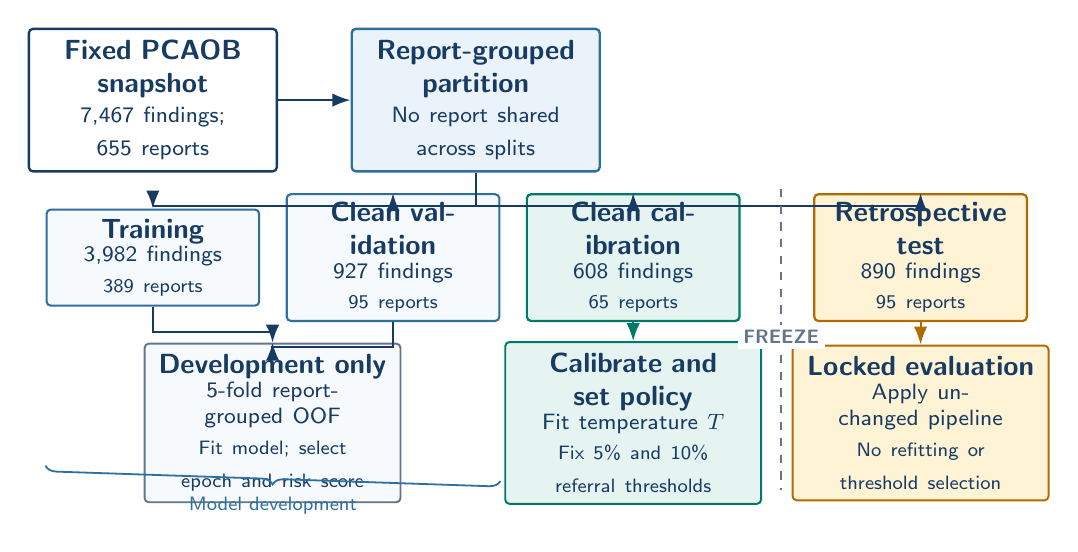
\begin{tikzpicture}[
    font=\sffamily,
    text=figNavy,
    dataflow/.style={-Latex, draw=figNavy, line width=0.78pt},
    sourcebox/.style={
      rectangle, rounded corners=1.5pt, draw=figNavy, fill=white,
      line width=0.85pt, minimum width=3.15cm, minimum height=1.15cm,
      text width=2.85cm, align=center, inner sep=4pt
    },
    splitbox/.style={
      rectangle, rounded corners=1.5pt, draw=figBlue, fill=figPale,
      line width=0.85pt, minimum width=3.15cm, minimum height=1.15cm,
      text width=2.85cm, align=center, inner sep=4pt
    },
    devcard/.style={
      rectangle, rounded corners=1.5pt, draw=figBlue, fill=figPaler,
      line width=0.75pt, minimum width=2.70cm, minimum height=1.22cm,
      text width=2.40cm, align=center, inner sep=3pt
    },
    calcard/.style={
      rectangle, rounded corners=1.5pt, draw=figTeal, fill=figTealPale,
      line width=0.8pt, minimum width=2.70cm, minimum height=1.22cm,
      text width=2.40cm, align=center, inner sep=3pt
    },
    testcard/.style={
      rectangle, rounded corners=1.5pt, draw=figAmber, fill=figAmberPale,
      line width=0.8pt, minimum width=2.70cm, minimum height=1.22cm,
      text width=2.40cm, align=center, inner sep=3pt
    },
    operation/.style={
      rectangle, rounded corners=1.5pt, draw=figSlate, fill=white,
      line width=0.7pt, minimum width=3.25cm, minimum height=1.36cm,
      text width=2.95cm, align=center, inner sep=4pt
    }
  ]
    \node[sourcebox] (snapshot) at (0,2.55) {
      \textbf{Fixed PCAOB snapshot}\\[-1pt]
      \footnotesize 7,467 findings; 655 reports};
    \node[splitbox] (partition) at (4.10,2.55) {
      \textbf{Report-grouped partition}\\[-1pt]
      \footnotesize No report shared across splits};

    \node[devcard] (train) at (0,0.55) {
      \textbf{Training}\\[-1pt]
      \footnotesize 3,982 findings\\[-1pt]
      \scriptsize 389 reports};
    \node[devcard] (valid) at (3.05,0.55) {
      \textbf{Clean validation}\\[-1pt]
      \footnotesize 927 findings\\[-1pt]
      \scriptsize 95 reports};
    \node[calcard] (cal) at (6.10,0.55) {
      \textbf{Clean calibration}\\[-1pt]
      \footnotesize 608 findings\\[-1pt]
      \scriptsize 65 reports};
    \node[testcard] (test) at (9.75,0.55) {
      \textbf{Retrospective test}\\[-1pt]
      \footnotesize 890 findings\\[-1pt]
      \scriptsize 95 reports};

    \node[operation, fill=figPaler] (develop) at (1.52,-1.55) {
      \textbf{Development only}\\[-1pt]
      \footnotesize 5-fold report-grouped OOF\\[-1pt]
      \scriptsize Fit model; select epoch and risk score};
    \node[operation, draw=figTeal, fill=figTealPale] (calibrate) at (6.10,-1.55) {
      \textbf{Calibrate and set policy}\\[-1pt]
      \footnotesize Fit temperature $T$\\[-1pt]
      \scriptsize Fix 5\% and 10\% referral thresholds};
    \node[operation, draw=figAmber, fill=figAmberPale] (evaluate) at (9.75,-1.55) {
      \textbf{Locked evaluation}\\[-1pt]
      \footnotesize Apply unchanged pipeline\\[-1pt]
      \scriptsize No refitting or threshold selection};

    \draw[dataflow] (snapshot) -- (partition);
    \coordinate (bus) at ($(partition.south)+(0,-0.43)$);
    \draw[draw=figNavy, line width=0.72pt] (partition.south) -- (bus);
    \draw[draw=figNavy, line width=0.72pt]
      (train.north |- bus) -- (test.north |- bus);
    \foreach \n in {train,valid,cal,test}{
      \draw[dataflow] (\n.north |- bus) -- (\n.north);
    }
    \draw[dataflow] (train.south) -- ++(0,-0.32) -| (develop.north);
    \draw[dataflow] (valid.south) -- ++(0,-0.32) -| (develop.north);
    \draw[dataflow, draw=figTeal] (cal.south) -- (calibrate.north);
    \draw[dataflow, draw=figAmber] (test.south) -- (evaluate.north);

    \coordinate (freezeTop) at (7.98,1.42);
    \coordinate (freezeBottom) at (7.98,-2.40);
    \draw[dashed, draw=figSlate, line width=0.85pt]
      (freezeTop) -- (freezeBottom);
    \node[fill=white, inner sep=2pt, font=\sffamily\scriptsize\bfseries,
      text=figSlate] at (7.98,-0.46) {FREEZE};

    \draw[decorate, decoration={brace, mirror, amplitude=4pt},
      draw=figBlue, line width=0.65pt]
      ($(train.south west)+(0,-2.02)$) -- ($(valid.south east)+(0,-2.02)$)
      node[midway, below=5pt, font=\sffamily\scriptsize, text=figBlue]
      {Model development};
  \end{tikzpicture}%
  }
  \caption{Leakage-controlled development and evaluation protocol. Reports,
  rather than individual findings, define the partitioning unit. Model fitting,
  epoch selection, and risk-score selection are confined to development data;
  temperature and operating thresholds are fixed on the independent calibration
  split. The dashed freeze boundary separates all selection decisions from the
  unchanged retrospective test evaluation. Counts for validation, calibration,
  and test refer to the clean evaluation subsets.}
  \label{fig:workflow}
\end{figure}

% =============================================================================
\section{Methods}
\label{sec:methods}
% =============================================================================

\subsection{Classical Sparse Baseline}

The classical sparse baseline combines word unigram and bigram TF--IDF features
with multinomial logistic regression. The vectorizer used a minimum document
frequency of 2, a maximum document frequency of 0.98, at most 50,000 features,
and sublinear term frequency. The classifier used balanced class weights and a
maximum of 3,000 iterations. Its inverse regularization strength was selected
from a prespecified grid using macro-F1 on the clean validation subset; for the
context input, the selected value was $C=64$. The model was then refitted on the
combined training and validation partitions. We refer to this model as a
classical sparse classifier, not as a small language model.

\subsection{General-Purpose Sentence-Embedding Baseline}

As a modern general-purpose representation baseline, we encoded each input with
\texttt{sentence-transformers/all-MiniLM-L6-v2}. Token sequences were truncated at
256 tokens, and token representations were combined by attention-mask mean
pooling followed by $L_2$ normalization. The encoder remained frozen. A balanced
logistic-regression classifier was trained on the resulting embeddings, with
$C$ selected on clean-validation macro-F1 ($C=4$ for the context input). This is
a frozen sentence-embedding linear probe rather than an end-to-end fine-tuned
Transformer.

\subsection{SEC-Domain Transformer}

The primary classifier was \texttt{nlpaueb/sec-bert-base}, resolved to Hugging
Face commit \texttt{d511591f5e74052afdab08f1f14c4ff2a1e55749}, with a 12-class
sequence-classification head. We
fine-tuned the complete network on \texttt{text\_context\_v2}. Sequences were
truncated at 256 tokens. Training used class-weighted cross-entropy, AdamW,
three epochs, a learning rate of $2\times10^{-5}$, weight decay of 0.01, a
physical batch size of 4, and four-step gradient accumulation for an effective
batch size of 16. A linear learning-rate schedule used a warm-up fraction of
0.1, gradients were clipped at 1.0, and the random seed was 20261002. The retained
epoch was selected exclusively by macro-F1 on the clean validation subset; neither
calibration nor test labels influenced weight or hyperparameter selection.
Gradient checkpointing reduced memory use without changing the model parameters
or effective batch size.

\subsection{Lexical-Cue Sensitivity Analysis}

We evaluated whether classifier performance depended on explicit audit-area
expressions and auditing-standard references. A deterministic transformation,
defined during dataset construction and applied identically across partitions,
replaced every phrase appearing in the official audit-area vocabulary with
\texttt{[AUDIT\_AREA]} and expressions such as ``AS 2301'' with
\texttt{[STANDARD\_REF]}. The target label remained an external supervision
variable and was never concatenated with the model input. Because an audit-area
term may be both a legitimate substantive feature and a direct lexical cue, this
experiment measures cue dependence rather than proving target leakage.

Two complementary conditions were used. First, the frozen canonical SEC-BERT,
trained on original text, was evaluated on both the original and masked versions
of the same 890 test findings. This paired stress test isolates sensitivity to an
input intervention but introduces a train--test representation shift. Second, a
separate SEC-BERT model was trained on masked training text, selected by masked
validation macro-F1, and evaluated on masked test text using the otherwise
unchanged three-epoch recipe. TF--IDF and MiniLM were compared under the same
matched original-training and masked-training design. For the paired SEC-BERT
stress test, 2,000 nonparametric bootstrap samples were drawn at the inspection-
report level to estimate intervals for the changes in accuracy and macro-F1.

\subsection{Probability Calibration}

For logits $z_i$ and temperature $T>0$, calibrated probabilities are
\begin{equation}
  p_T(y\mid x_i)=\operatorname{softmax}\!\left(\frac{z_i}{T}\right).
  \label{eq:temperature}
\end{equation}

A single scalar temperature was fitted by minimizing multiclass negative
log-likelihood on the 608 clean calibration findings. The resulting frozen value
was $T=1.1517754200$. Because division by a positive scalar preserves logit order,
temperature scaling changed uncertainty estimates but not the predicted class.

\subsection{Risk Scores}

Let $p_{(1)}(x_i)$ and $p_{(2)}(x_i)$ denote the largest and second-largest
probabilities available at a given decision stage. The top-two margin is
\begin{equation}
  m(x_i)=p_{(1)}(x_i)-p_{(2)}(x_i).
  \label{eq:margin}
\end{equation}

We compared three directly derived score families: maximum confidence
$c(x_i)=p_{(1)}(x_i)$, top-two margin $m(x_i)$, and predictive entropy
\begin{equation}
  H(x_i)=-\sum_{y\in\mathcal{Y}}p(y\mid x_i)\log p(y\mid x_i).
\end{equation}
We also evaluated class-aware logistic error models using uncertainty, text,
context-quality, topic, and baseline-disagreement features. These learned scores
were generated by report-grouped cross-fitting so that the risk estimate for a
finding was produced without training on its report. Score-family selection was
performed on 4,613 clean out-of-fold development predictions using their raw
softmax probabilities ($T=1$). Top-two margin was selected before the calibration
split was opened. After the scalar temperature had been fitted on calibration,
the same margin functional form was applied to $p_T$ and only its two operating
thresholds were selected. Thus, calibration labels changed neither the selected
score family nor the base classifier.

\subsection{Frozen Selective Policies}

After fitting the temperature, we used the calibration split only to select two
operating points. The high-coverage policy abstains when the calibrated margin is
below 0.5269052934, corresponding to approximately 5\% calibration abstention.
The conservative policy abstains below 0.8157442331, corresponding to approximately
10\% calibration abstention. Both thresholds, the comparison operator, the
temperature, the model recipe, and all outcome definitions were frozen before
retrospective test evaluation.

% =============================================================================
\section{Experimental Design}
\label{sec:experimental-design}
% =============================================================================

\subsection{PCAOB Data Source and Provenance}

The source was the official downloadable PCAOB Part I.A inspection-findings file,
retrieved on September 27, 2026. The immutable source snapshot has SHA-256 digest
\texttt{af543784fa73475741e20324ce451b1de1df96fe4a826fd292b1f9aa4b7c96d7}.
It contains inspection years 2018--2025. We aggregated 14,043 source rows into
7,467 finding-level records across 655 inspection reports and 392 firms. All
subsequent transformations were derived from this snapshot.

\subsection{Eligibility, Cleaning, and Label Construction}

The modeling population retained 6,607 findings with one explicit study label,
covering 650 reports and 391 firms. We excluded 615 multi-label findings because
the primary experiment is single-label classification, and 245 cases with
deterministically identified target conflicts were removed upstream. Normalized
text revealed 268 exact-duplicate groups, of which 169 had more than one observed
label set; duplicate and leakage controls were recorded before model fitting.

Some finding fragments depend on antecedent text in the same report. Of 1,295
findings flagged as context-dependent, 366 were safely restored using text tied to
the same report, issuer, and official audit area. The remaining 929 were retained
with an unresolved-context flag rather than filled speculatively. The same
deterministic label map, text construction, duplicate rules, and context flags
were applied to every partition.

\begin{table}[t]
  \centering
  \caption{Dataset construction and report-grouped partitions. Clean counts exclude records flagged by the prespecified evaluation-quality rules.}
  \label{tab:data}
  \begin{tabular}{lrr}
    \toprule
    Stage or partition & Records/findings & Reports \\
    \midrule
    Raw PCAOB source rows & 14,043 & 655 \\
    Aggregated finding-level records & 7,467 & 655 \\
    Single-label modeling population & 6,607 & 650 \\
    Training split & 3,982 & 389 \\
    Validation split (clean) & 927 & 95 \\
    Calibration split (clean) & 608 & 65 \\
    Retrospective test (clean) & 890 & 95 \\
    Development OOF (clean) & 4,613 & 477 \\
    \bottomrule
  \end{tabular}
\end{table}

\subsection{Report-Grouped Partitions}

The fixed report-grouped split contained 3,982 training, 992 validation, 666
calibration, and 967 test findings. Application of the prespecified clean-evaluation
flag yielded 927 validation, 608 calibration, and 890 retrospective-test findings.
No inspection report crossed partitions. The report, rather than the individual
finding, was therefore the unit used to prevent direct information leakage and to
form uncertainty intervals. The test partition is a held-out report-grouped
retrospective test, not a prospective temporal holdout.

\subsection{Development, Calibration, and Freezing Sequence}

The experiment followed a fixed chronology. First, train, validation, calibration,
and test reports were locked. Second, five-fold report-grouped cross-fitting on the
combined training and validation partitions produced 4,613 clean out-of-fold
predictions from 477 reports. These predictions were used to compare uncertainty
scores and select margin as the routing score. Third, the canonical SEC-BERT was
trained on the training partition and its epoch was selected on clean validation
macro-F1. Fourth, logits from the independent calibration partition were used to
fit the temperature and choose the two thresholds. We then froze the checkpoint
recipe, preprocessing, taxonomy, temperature, score, thresholds, and metrics.
Only after this freeze was the unchanged pipeline applied to the 890-case
retrospective test. A future temporal confirmation is reserved for official reports
that first appear after the source snapshot.

\subsection{Comparison Hierarchy and Decision Logic}

The experiments follow a staged comparison so that each result answers one
decision before the next stage is introduced. First, the three classifier
families are compared under identical report-grouped partitions to identify the
strongest base predictor. Second, uncertainty and learned risk scores are
compared only for that frozen predictor using development out-of-fold outcomes.
Third, temperature and two operating thresholds are estimated on the independent
calibration partition and transferred unchanged to the retrospective test. This
hierarchy keeps classifier selection, probability calibration, error ranking,
and release control as distinct claims.

\subsection{Outcome Metrics}

Ordinary classification performance was summarized by accuracy, macro-F1,
balanced accuracy, and per-class recall. Probability quality was evaluated using
negative log-likelihood, the multiclass Brier score, and expected calibration error
with ten equal-width confidence bins. Selective performance was evaluated by
coverage, abstention rate, selective accuracy and risk, error capture, abstention
precision, and the full risk--coverage curve. Reporting both queue size and queue
yield prevents a low-error automatic subset from being interpreted without its
associated verification burden.

\subsection{Statistical Inference}

Confidence intervals and paired model comparisons were obtained by nonparametric
bootstrap resampling of inspection reports, retaining all findings belonging to a
sampled report. The frozen retrospective analysis used 5,000 bootstrap replicates.
Sample-level binomial bounds were used only as a development diagnostic; they are
not presented as a formal selective-risk guarantee because findings within one
report are dependent.

\subsection{Temporal Confirmation Protocol}

The temporal protocol fixes the model recipe and weights, text preprocessing,
12-class mapping, temperature, top-two-margin score, both thresholds, eligibility
rules, and all reported metrics. The confirmatory set will include only inspection
reports that first become available after the September 27, 2026 snapshot. These
reports may not be used for retraining, recalibration, threshold reselection, or
taxonomy revision. If no eligible new reports are available, the study reports the
protocol as pending rather than substituting the retrospective split for a temporal
result.

\subsection{Reproducibility}

The reproducibility package records executable source code, configuration files,
the source-data manifest and digest, split assignments, out-of-fold predictions,
calibration and test logits, training histories, random seeds, and frozen operating
points. SEC-BERT training was run on an NVIDIA GeForce RTX 3050 Laptop GPU with
Python 3.13.1, PyTorch 2.11.0 with CUDA 12.8, and Transformers 5.8.0. The masking run exported
the complete environment, predictions for all three sensitivity conditions, and
a SHA-256 manifest for the original and masked model files. The two weight
archives are preserved locally with their tokenizer files, training configurations,
predictions, and per-file hashes. The canonical archive has SHA-256 digest
\texttt{46AF65999D260CC5A100AE4F6DE99B6AF8E4798F67CE75160074E24F54396045};
the masked-model archive has digest
\texttt{2A74CA96DCF023B7B671681988C24C3319C50C27F531D469274052D46CD3108C}.

% =============================================================================
\section{Results}
\label{sec:results}
% =============================================================================

\subsection{Dataset Characteristics and Quality Controls}

The official source contained 14,043 rows, which were aggregated into 7,467
finding-level records. After restricting the primary task to explicit single-label
cases and applying the deterministic target-conflict rules, the modeling population
contained 6,607 findings from 650 inspection reports and 391 registered firms.
The 12-class distribution was imbalanced. Revenue and Receivables was the largest
class ($n=2{,}298$), whereas Income Taxes ($n=66$), Expenses, Compensation and
Benefits ($n=102$), and Related Parties and Significant Transactions ($n=156$)
were the smallest classes. This imbalance motivated the use of macro-F1, balanced
accuracy, class-weighted training, and per-class analysis in addition to accuracy.

The construction audit identified 615 multi-label findings and 245 deterministic
target conflicts outside the primary single-label task. It also found 268 groups
of exactly duplicated normalized narratives; 169 of these groups were associated
with more than one label set. Report-grouped partitioning and the clean-evaluation
rules were therefore necessary to reduce direct template leakage. Among 1,295
findings flagged as potentially dependent on earlier report text, 366 received a
deterministically matched preamble and 929 remained flagged as unresolved. In the
clean retrospective test, 698 findings were self-contained, 60 had restored
context, and 132 retained an unresolved-context flag. These flags describe
observable data conditions, not expert-adjudicated ambiguity.

\subsection{RQ1: Classification Performance}

Table~\ref{tab:model-comparison} compares the three principal representations on
the same 890-case clean retrospective test. The frozen MiniLM representation with
a linear classifier attained 0.8607 accuracy and 0.7932 macro-F1. The classical
TF--IDF classifier was stronger, reaching 0.9124 accuracy and 0.8536 macro-F1.
End-to-end fine-tuning of SEC-BERT produced the highest point estimates: 0.9337
accuracy, 0.9021 macro-F1, and 0.9058 balanced accuracy. Thus, the main gain was
not obtained merely by replacing sparse features with a frozen dense embedding;
the strongest observed pipeline used end-to-end task adaptation of the
domain-pretrained encoder. Because the general-purpose MiniLM representation was
frozen, this comparison does not isolate domain pretraining from full-network
fine-tuning.

The SEC-BERT accuracy estimate exceeded the TF--IDF/context baseline by 2.13
percentage points. However, the report-cluster bootstrap 95\% interval for this
paired difference was $[-0.89,5.26]$ percentage points. The result therefore
supports SEC-BERT as the strongest observed model and the appropriate classifier
for subsequent selective analysis, but it does not establish statistically
conclusive superiority over TF--IDF in the available reports.

\begin{table}[t]
  \centering
  \caption{Classification performance on the clean report-grouped retrospective test set.}
  \label{tab:model-comparison}
  \begin{tabular}{lccc}
    \toprule
    Model & Accuracy & Macro-F1 & Balanced accuracy \\
    \midrule
    TF-IDF + logistic regression & 0.9124 & 0.8536 & 0.8460 \\
    MiniLM embedding baseline & 0.8607 & 0.7932 & 0.8116 \\
    SEC-BERT & 0.9337 & 0.9021 & 0.9058 \\
    \bottomrule
  \end{tabular}
\end{table}

The frozen canonical SEC-BERT attained 0.9337 accuracy, 0.9021 macro-F1, and
0.9058 balanced accuracy on the 890 test findings. When this fixed model instead
received the masked versions of those findings, accuracy fell to 0.3809,
macro-F1 to 0.2787, and balanced accuracy to 0.3117. Predictions changed for
61.91\% of findings. The paired changes were $-55.28$ percentage points in
accuracy (95\% report-cluster bootstrap interval $[-60.34,-50.36]$) and $-62.34$
points in macro-F1 ($[-70.04,-58.95]$). Thus, the canonical model was highly
sensitive to removal of
explicit audit-area and standards cues.

Training SEC-BERT directly on the masked input recovered performance to 0.6708
accuracy, 0.5332 macro-F1, and 0.5463 balanced accuracy. This recovery shows that
the remaining context contained learnable signal, but it did not restore the
original-text performance. Under matched training and evaluation
(Table~\ref{tab:masking-sensitivity}), masked SEC-BERT had a lower macro-F1 point
estimate than masked TF--IDF (0.5332 versus 0.5585), while exceeding masked
MiniLM (0.4969). No paired interval was estimated for the difference between the
separately trained masked models, so these comparisons are descriptive rather
than claims of statistical superiority.

\begin{table}[t]
  \centering
  \caption{Lexical-cue sensitivity on the 890-case retrospective test. The
  first three rows compare matched original-text and masked-text training and
  evaluation. The final row is an input-shift stress test using the fixed
  original-text SEC-BERT without masked-input retraining.}
  \label{tab:masking-sensitivity}
  \begin{tabular}{lrrr}
    \toprule
    Model and condition & Original macro-F1 & Masked macro-F1 & Change (pp) \\
    \midrule
    TF--IDF, matched training & 0.8536 & 0.5585 & $-29.51$ \\
    MiniLM, matched training & 0.7932 & 0.4969 & $-29.63$ \\
    SEC-BERT, matched training & 0.9021 & 0.5332 & $-36.89$ \\
    SEC-BERT, no masked retraining & 0.9021 & 0.2787 & $-62.34$ \\
    \bottomrule
  \end{tabular}
\end{table}

\begin{figure}[htbp]
  \centering
  \resizebox{\textwidth}{!}{%
  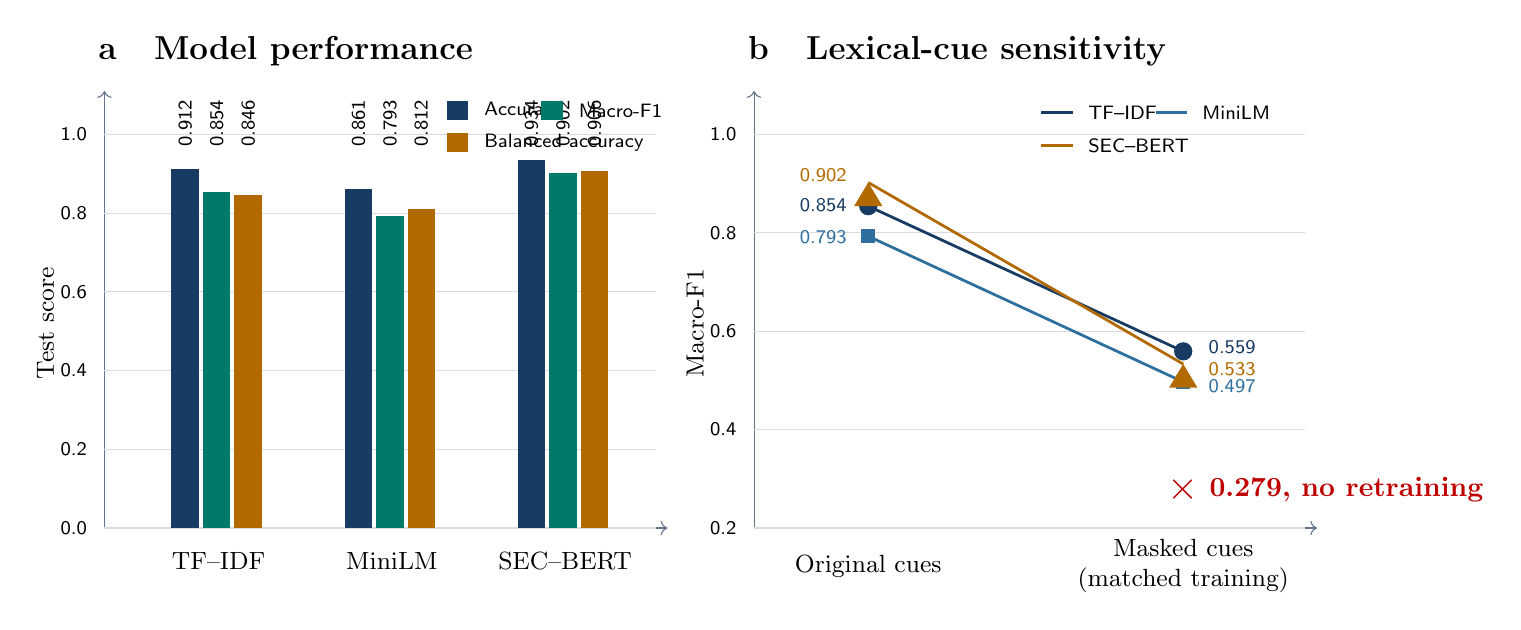
\begin{tikzpicture}[font=\sffamily\scriptsize]
    \begin{scope}
      \node[font=\bfseries\large, anchor=west] at (-0.2,6.05) {a\quad Model performance};
      \draw[->, draw=figSlate] (0,0) -- (0,5.55);
      \draw[->, draw=figSlate] (0,0) -- (7.15,0);
      \foreach \y/\lab in {0/0.0,1/0.2,2/0.4,3/0.6,4/0.8,5/1.0}{
        \draw[figSlate!25] (0,\y) -- (7,\y);
        \node[anchor=east] at (-0.10,\y) {\lab};
      }
      \node[rotate=90, font=\small] at (-0.75,2.6) {Test score};
      \foreach \x/\lab in {1.45/TF--IDF,3.65/MiniLM,5.85/SEC--BERT}{
        \node[font=\small] at (\x,-0.42) {\lab};
      }
      \fill[figNavy] (0.85,0) rectangle (1.20,4.562);
      \fill[figTeal] (1.25,0) rectangle (1.60,4.268);
      \fill[figAmber] (1.65,0) rectangle (2.00,4.230);
      \fill[figNavy] (3.05,0) rectangle (3.40,4.304);
      \fill[figTeal] (3.45,0) rectangle (3.80,3.966);
      \fill[figAmber] (3.85,0) rectangle (4.20,4.058);
      \fill[figNavy] (5.25,0) rectangle (5.60,4.669);
      \fill[figTeal] (5.65,0) rectangle (6.00,4.511);
      \fill[figAmber] (6.05,0) rectangle (6.40,4.529);
      \foreach \x/\lab in {1.025/0.912,1.425/0.854,1.825/0.846,3.225/0.861,3.625/0.793,4.025/0.812,5.425/0.934,5.825/0.902,6.225/0.906}{
        \node[rotate=90, anchor=west] at (\x,4.72) {\lab};
      }
      \fill[figNavy] (4.35,5.18) rectangle (4.62,5.42);
      \node[anchor=west] at (4.70,5.30) {Accuracy};
      \fill[figTeal] (5.55,5.18) rectangle (5.82,5.42);
      \node[anchor=west] at (5.90,5.30) {Macro-F1};
      \fill[figAmber] (4.35,4.78) rectangle (4.62,5.02);
      \node[anchor=west] at (4.70,4.90) {Balanced accuracy};
    \end{scope}
    \begin{scope}[xshift=8.25cm]
      \node[font=\bfseries\large, anchor=west] at (-0.2,6.05) {b\quad Lexical-cue sensitivity};
      \draw[->, draw=figSlate] (0,0) -- (0,5.55);
      \draw[->, draw=figSlate] (0,0) -- (7.15,0);
      \foreach \y/\lab in {0/0.2,1.25/0.4,2.5/0.6,3.75/0.8,5/1.0}{
        \draw[figSlate!25] (0,\y) -- (7,\y);
        \node[anchor=east] at (-0.10,\y) {\lab};
      }
      \node[rotate=90, font=\small] at (-0.75,2.6) {Macro-F1};
      \node[font=\small] at (1.45,-0.48) {Original cues};
      \node[font=\small, align=center] at (5.45,-0.48) {Masked cues\\(matched training)};
      \draw[figNavy, line width=1.0pt] (1.45,4.088) -- (5.45,2.244);
      \draw[figBlue, line width=1.0pt] (1.45,3.706) -- (5.45,1.856);
      \draw[figAmber, line width=1.0pt] (1.45,4.388) -- (5.45,2.083);
      \fill[figNavy] (1.45,4.088) circle (3.3pt); \fill[figNavy] (5.45,2.244) circle (3.3pt);
      \fill[figBlue] (1.36,3.617) rectangle (1.54,3.795); \fill[figBlue] (5.36,1.767) rectangle (5.54,1.945);
      \fill[figAmber] (1.45,4.388) -- +(0.18,-0.30) -- +(-0.18,-0.30) -- cycle;
      \fill[figAmber] (5.45,2.083) -- +(0.18,-0.30) -- +(-0.18,-0.30) -- cycle;
      \node[text=figNavy, anchor=east] at (1.30,4.10) {0.854};
      \node[text=figBlue, anchor=east] at (1.30,3.70) {0.793};
      \node[text=figAmber, anchor=east] at (1.30,4.48) {0.902};
      \node[text=figNavy, anchor=west] at (5.65,2.30) {0.559};
      \node[text=figBlue, anchor=west] at (5.65,1.80) {0.497};
      \node[text=figAmber, anchor=west] at (5.65,2.02) {0.533};
      \node[text=red!75!black, font=\bfseries\Large] at (5.45,0.49) {$\times$};
      \node[text=red!75!black, anchor=west, font=\bfseries] at (5.66,0.49) {0.279, no retraining};
      \draw[figNavy, line width=1pt] (3.65,5.28)--(4.05,5.28); \node[anchor=west] at (4.12,5.28) {TF--IDF};
      \draw[figBlue, line width=1pt] (5.10,5.28)--(5.50,5.28); \node[anchor=west] at (5.57,5.28) {MiniLM};
      \draw[figAmber, line width=1pt] (3.65,4.86)--(4.05,4.86); \node[anchor=west] at (4.12,4.86) {SEC--BERT};
    \end{scope}
  \end{tikzpicture}%
  }
  \caption{Classifier quality and dependence on explicit audit-area cues.
  \textbf{(a)} Accuracy, macro-F1, and balanced accuracy for the three model
  families on the same 890-case clean retrospective test. SEC-BERT produced the
  strongest point estimate for every metric, whereas the frozen MiniLM baseline
  did not improve on the sparse TF--IDF classifier. \textbf{(b)} Macro-F1 before
  and after masking explicit audit-area expressions and standards references
  under matched training conditions. TF--IDF, MiniLM, and SEC-BERT lost 29.5,
  29.6, and 36.9 percentage points, respectively. The red cross shows the more
  severe input-shift stress test in which the original-text SEC-BERT received
  masked test text without retraining (macro-F1 0.2787). Masking removes both
  possible target cues and substantively meaningful account terms; the panel
  therefore measures lexical-cue dependence rather than proving label leakage.}
  \label{fig:model-comparison-sensitivity}
\end{figure}

\subsection{RQ2: Error-Ranking Performance}

Risk scores were first compared on 4,613 clean report-grouped out-of-fold
predictions, which contained 305 label disagreements. The learned class-aware
logistic score discriminated errors well in a threshold-free sense
(ROC--AUC $=0.9043$; average precision $=0.4200$ at an error prevalence of
0.0661). Nevertheless, its area under the discrete risk--coverage curve was
0.01012, compared with 0.00996 for maximum confidence, 0.00999 for entropy,
and 0.00987 for top-two margin; lower values are preferable. Random ranking
produced 0.07049, while the non-deployable oracle bound was 0.00224.

The same ordering was visible at the prespecified 5\% referral budget. Margin
retained 94.99\% coverage with 0.9569 selective accuracy, captured 38.03\% of
all disagreements, and yielded 50.22\% abstention precision. Confidence,
entropy, and the learned score achieved selective accuracies of 0.9566, 0.9564,
and 0.9562, respectively, whereas random referral remained at 0.9338. The
differences among the uncertainty-based scores were small, but the learned
router did not improve the fixed-budget outcome. We therefore selected margin
on development data as the primary score before examining calibration outcomes.
This supports a simple error-ranking rule; it does not provide a formal bound on
future selective risk.

\subsection{Calibration and Threshold Freezing}

On the independent 608-case calibration split, the fitted temperature was
$T=1.15178$. Temperature scaling reduced negative log-likelihood from 0.3206 to
0.3113, the multiclass Brier score from 0.1273 to 0.1245, and ten-bin expected
calibration error from 0.0459 to 0.0311 (Table~\ref{tab:calibration}). Accuracy
and macro-F1 remained 0.9293 and 0.9174 because scalar temperature scaling does
not change the ordering of class logits. On the retrospective test, the same
frozen transformation reduced expected calibration error from 0.0335 to 0.0224
and negative log-likelihood from 0.3076 to 0.2965. The calibrated margin was then
used to freeze the two prespecified operating points before retrospective test
evaluation.

\begin{table}[t]
  \centering
  \caption{Probability calibration on the independent calibration split.}
  \label{tab:calibration}
  \begin{tabular}{lccccc}
    \toprule
    Method & Accuracy & Macro-F1 & NLL & Brier & ECE \\
    \midrule
    Raw probabilities & 0.9293 & 0.9174 & 0.3206 & 0.1273 & 0.0459 \\
    Temperature scaled & 0.9293 & 0.9174 & 0.3113 & 0.1245 & 0.0311 \\
    \bottomrule
  \end{tabular}
\end{table}

\begin{figure}[htbp]
  \centering
  \resizebox{\textwidth}{!}{%
  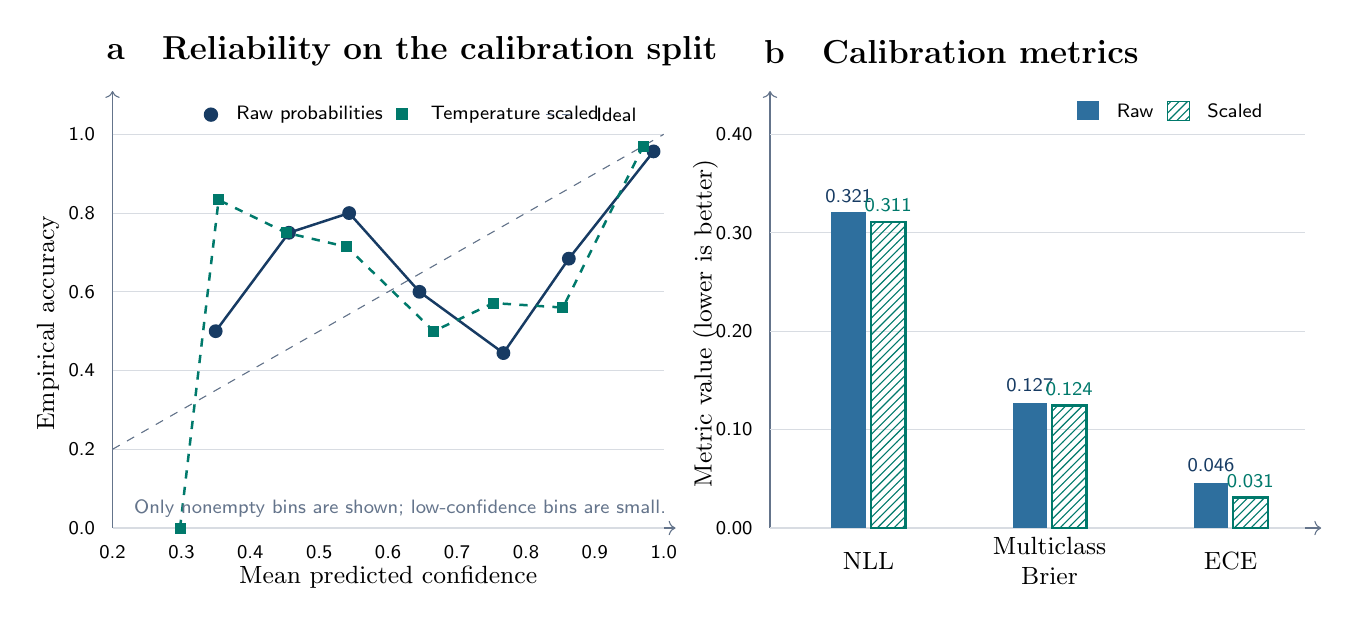
\begin{tikzpicture}[font=\sffamily\scriptsize]
    \begin{scope}
      \node[font=\bfseries\large, anchor=west] at (-0.2,6.05) {a\quad Reliability on the calibration split};
      \draw[->, draw=figSlate] (0,0) -- (0,5.55);
      \draw[->, draw=figSlate] (0,0) -- (7.15,0);
      \foreach \y/\lab in {0/0.0,1/0.2,2/0.4,3/0.6,4/0.8,5/1.0}{
        \draw[figSlate!25] (0,\y) -- (7,\y); \node[anchor=east] at (-0.10,\y) {\lab};
      }
      \foreach \x/\lab in {0/0.2,0.875/0.3,1.75/0.4,2.625/0.5,3.5/0.6,4.375/0.7,5.25/0.8,6.125/0.9,7/1.0}{
        \node[anchor=north] at (\x,-0.10) {\lab};
      }
      \node[font=\small] at (3.5,-0.62) {Mean predicted confidence};
      \node[rotate=90, font=\small] at (-0.82,2.6) {Empirical accuracy};
      \draw[figSlate, dashed] (0,1.0) -- (7,5);
      \draw[figNavy, line width=0.9pt]
        (1.310,2.500)--(2.240,3.750)--(3.005,4.000)--(3.898,3.000)--(4.964,2.222)--(5.795,3.421)--(6.871,4.783);
      \draw[figTeal, dashed, line width=0.9pt]
        (0.857,0.000)--(1.347,4.167)--(2.205,3.750)--(2.976,3.571)--(4.079,2.500)--(4.837,2.857)--(5.720,2.800)--(6.740,4.851);
      \foreach \x/\y in {1.310/2.500,2.240/3.750,3.005/4.000,3.898/3.000,4.964/2.222,5.795/3.421,6.871/4.783}{\fill[figNavy] (\x,\y) circle (2.5pt);}
      \foreach \x/\y in {0.857/0.000,1.347/4.167,2.205/3.750,2.976/3.571,4.079/2.500,4.837/2.857,5.720/2.800,6.740/4.851}{\fill[figTeal] (\x-0.07,\y-0.07) rectangle (\x+0.07,\y+0.07);}
      \fill[figNavy] (1.25,5.25) circle (2.6pt); \node[anchor=west] at (1.45,5.25) {Raw probabilities};
      \fill[figTeal] (3.60,5.18) rectangle (3.75,5.33); \node[anchor=west] at (3.92,5.25) {Temperature scaled};
      \draw[figSlate, dashed] (5.50,5.25)--(5.92,5.25); \node[anchor=west] at (6.02,5.25) {Ideal};
      \node[text=figSlate, anchor=west] at (0.15,0.25) {Only nonempty bins are shown; low-confidence bins are small.};
    \end{scope}
    \begin{scope}[xshift=8.35cm]
      \node[font=\bfseries\large, anchor=west] at (-0.2,6.05) {b\quad Calibration metrics};
      \draw[->, draw=figSlate] (0,0) -- (0,5.55);
      \draw[->, draw=figSlate] (0,0) -- (7.0,0);
      \foreach \y/\lab in {0/0.00,1.25/0.10,2.5/0.20,3.75/0.30,5/0.40}{
        \draw[figSlate!25] (0,\y)--(6.8,\y); \node[anchor=east] at (-0.10,\y) {\lab};
      }
      \node[rotate=90, font=\small] at (-0.82,2.6) {Metric value (lower is better)};
      \node[font=\small] at (1.25,-0.42) {NLL};
      \node[font=\small, align=center] at (3.55,-0.42) {Multiclass\\Brier};
      \node[font=\small] at (5.85,-0.42) {ECE};
      \fill[figBlue] (0.78,0) rectangle (1.22,4.008);
      \draw[figTeal, line width=0.8pt, pattern=north east lines, pattern color=figTeal] (1.28,0) rectangle (1.72,3.891);
      \fill[figBlue] (3.08,0) rectangle (3.52,1.591);
      \draw[figTeal, line width=0.8pt, pattern=north east lines, pattern color=figTeal] (3.58,0) rectangle (4.02,1.556);
      \fill[figBlue] (5.38,0) rectangle (5.82,0.574);
      \draw[figTeal, line width=0.8pt, pattern=north east lines, pattern color=figTeal] (5.88,0) rectangle (6.32,0.389);
      \node[text=figNavy] at (1.00,4.22) {0.321}; \node[text=figTeal] at (1.50,4.10) {0.311};
      \node[text=figNavy] at (3.30,1.81) {0.127}; \node[text=figTeal] at (3.80,1.77) {0.124};
      \node[text=figNavy] at (5.60,0.80) {0.046}; \node[text=figTeal] at (6.10,0.60) {0.031};
      \fill[figBlue] (3.90,5.18) rectangle (4.18,5.42); \node[anchor=west] at (4.28,5.30) {Raw};
      \draw[figTeal, pattern=north east lines, pattern color=figTeal] (5.05,5.18) rectangle (5.33,5.42); \node[anchor=west] at (5.43,5.30) {Scaled};
    \end{scope}
  \end{tikzpicture}%
  }
  \caption{Probability calibration on the independent 608-case calibration
  split. \textbf{(a)} Reliability curves before and after fitting the scalar
  temperature. Only nonempty bins are shown; the visibly volatile low-confidence
  bins contain few findings and should
  not be interpreted without regard to their small sample sizes. The dashed
  diagonal denotes perfect calibration. \textbf{(b)} Negative log-likelihood
  (NLL), multiclass Brier score, and ten-bin expected calibration error (ECE).
  Temperature scaling preserved class predictions while reducing all three
  calibration metrics, with the largest relative reduction in ECE.}
  \label{fig:probability-calibration}
\end{figure}

\subsection{RQ3: Selective-Automation Performance}

Without abstention, SEC-BERT agreed with the PCAOB-derived labels on 93.37\% of
the retrospective test. The frozen high-coverage policy referred 32 of 890
findings (3.60\%) and automatically accepted the remaining 96.40\%. Agreement
within the accepted subset was 95.22\% (report-cluster 95\% interval
$[93.38\%,97.13\%]$). The queue contained 18 of the model's 59 disagreements,
for an error-capture rate of 30.51\% and an abstention precision of 56.25\%.

The conservative policy referred 63 findings (7.08\%), leaving 92.92\% for
automatic acceptance. Selective accuracy rose to 96.61\% (report-cluster 95\%
interval $[94.61\%,98.26\%]$), and the queue captured 31 of 59 disagreements
(52.54\%) with 49.21\% abstention precision. Thus, approximately twice the
verification volume captured substantially more disagreements. Neither
selective accuracy is an end-to-end human--AI accuracy: the study did not observe
whether referred cases were reviewed or corrected.

\begin{table}[t]
  \centering
  \caption{Frozen selective-automation policies on the retrospective test set.}
  \label{tab:operating-points}
  \begin{tabular}{lccccc}
    \toprule
    Policy & Abstention & Coverage & Sel. accuracy & Error capture & Abst. precision \\
    \midrule
    Full automation & 0.0000 & 1.0000 & 0.9337 & 0.0000 & -- \\
    High-coverage policy & 0.0360 & 0.9640 & 0.9522 & 0.3051 & 0.5625 \\
    Conservative policy & 0.0708 & 0.9292 & 0.9661 & 0.5254 & 0.4921 \\
    \bottomrule
  \end{tabular}
\end{table}

\begin{figure}[htbp]
  \centering
  \resizebox{\textwidth}{!}{%
  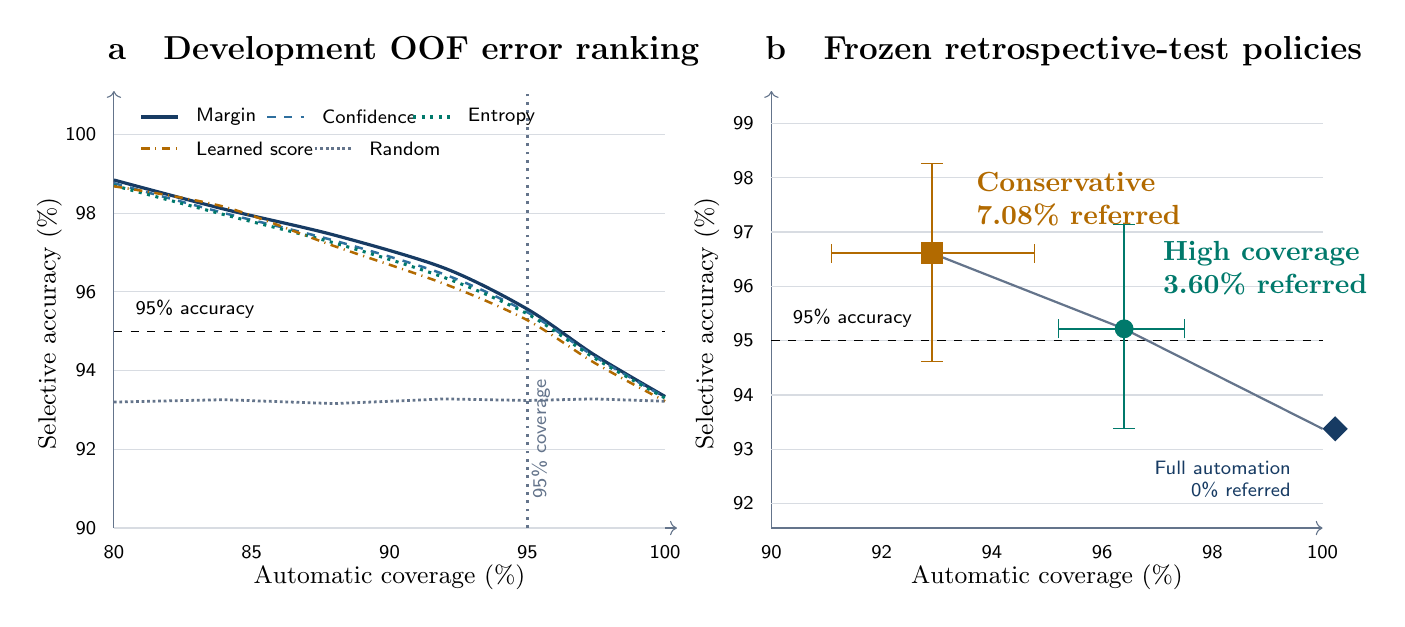
\begin{tikzpicture}[font=\sffamily\scriptsize]
    \begin{scope}
      \node[font=\bfseries\large, anchor=west] at (-0.2,6.05) {a\quad Development OOF error ranking};
      \draw[->, draw=figSlate] (0,0) -- (0,5.55);
      \draw[->, draw=figSlate] (0,0) -- (7.15,0);
      \foreach \x/\lab in {0/80,1.75/85,3.5/90,5.25/95,7/100}{\node[anchor=north] at (\x,-0.10) {\lab};}
      \foreach \y/\lab in {0/90,1/92,2/94,3/96,4/98,5/100}{\draw[figSlate!25] (0,\y)--(7,\y);\node[anchor=east] at (-0.10,\y) {\lab};}
      \node[font=\small] at (3.5,-0.62) {Automatic coverage (\%)};
      \node[rotate=90, font=\small] at (-0.82,2.6) {Selective accuracy (\%)};
      \draw[black, dashed] (0,2.5)--(7,2.5); \node[anchor=west] at (0.15,2.78) {95\% accuracy};
      \draw[figSlate, dotted, line width=1pt] (5.25,0)--(5.25,5.55);
      \node[rotate=90, text=figSlate, anchor=west] at (5.42,0.25) {95\% coverage};
      \draw[figNavy, line width=1.15pt] plot[smooth] coordinates {(0,4.42)(1.4,4.05)(2.8,3.72)(4.2,3.30)(5.25,2.78)(6.1,2.20)(7,1.67)};
      \draw[figBlue, dashed, line width=0.9pt] plot[smooth] coordinates {(0,4.38)(1.4,4.00)(2.8,3.65)(4.2,3.22)(5.25,2.74)(6.1,2.18)(7,1.66)};
      \draw[figTeal, dotted, line width=1.1pt] plot[smooth] coordinates {(0,4.35)(1.4,3.98)(2.8,3.62)(4.2,3.18)(5.25,2.72)(6.1,2.16)(7,1.65)};
      \draw[figAmber, dash dot, line width=0.9pt] plot[smooth] coordinates {(0,4.34)(1.4,4.08)(2.8,3.58)(4.2,3.10)(5.25,2.64)(6.1,2.10)(7,1.61)};
      \draw[figSlate, densely dotted, line width=1pt] plot coordinates {(0,1.60)(1.4,1.63)(2.8,1.58)(4.2,1.64)(5.25,1.62)(6.1,1.64)(7,1.61)};
      \draw[figNavy, line width=1.1pt] (0.35,5.22)--(0.82,5.22); \node[anchor=west] at (0.92,5.22) {Margin};
      \draw[figBlue, dashed, line width=1pt] (1.95,5.22)--(2.42,5.22); \node[anchor=west] at (2.52,5.22) {Confidence};
      \draw[figTeal, dotted, line width=1.1pt] (3.80,5.22)--(4.27,5.22); \node[anchor=west] at (4.37,5.22) {Entropy};
      \draw[figAmber, dash dot, line width=1pt] (0.35,4.82)--(0.82,4.82); \node[anchor=west] at (0.92,4.82) {Learned score};
      \draw[figSlate, densely dotted, line width=1pt] (2.55,4.82)--(3.02,4.82); \node[anchor=west] at (3.12,4.82) {Random};
    \end{scope}
    \begin{scope}[xshift=8.35cm]
      \node[font=\bfseries\large, anchor=west] at (-0.2,6.05) {b\quad Frozen retrospective-test policies};
      \draw[->, draw=figSlate] (0,0) -- (0,5.55);
      \draw[->, draw=figSlate] (0,0) -- (7.0,0);
      \foreach \x/\lab in {0/90,1.4/92,2.8/94,4.2/96,5.6/98,7/100}{\node[anchor=north] at (\x,-0.10) {\lab};}
      \foreach \y/\lab in {0.31/92,1.00/93,1.69/94,2.38/95,3.07/96,3.76/97,4.45/98,5.14/99}{\draw[figSlate!25] (0,\y)--(7,\y);\node[anchor=east] at (-0.10,\y) {\lab};}
      \node[font=\small] at (3.5,-0.62) {Automatic coverage (\%)};
      \node[rotate=90, font=\small] at (-0.82,2.6) {Selective accuracy (\%)};
      \draw[black, dashed] (0,2.38)--(7,2.38); \node[anchor=west] at (0.15,2.66) {95\% accuracy};
      \draw[figSlate, line width=0.8pt] (2.04,3.49)--(4.48,2.53)--(7,1.26);
      \draw[figAmber, line width=0.9pt] (2.04,2.11)--(2.04,4.63); \draw[figAmber] (1.90,2.11)--(2.18,2.11) (1.90,4.63)--(2.18,4.63);
      \draw[figAmber, line width=0.9pt] (0.76,3.49)--(3.34,3.49); \draw[figAmber] (0.76,3.37)--(0.76,3.61) (3.34,3.37)--(3.34,3.61);
      \fill[figAmber] (1.90,3.35) rectangle (2.18,3.63);
      \draw[figTeal, line width=0.9pt] (4.48,1.26)--(4.48,3.85); \draw[figTeal] (4.34,1.26)--(4.62,1.26) (4.34,3.85)--(4.62,3.85);
      \draw[figTeal, line width=0.9pt] (3.65,2.53)--(5.25,2.53); \draw[figTeal] (3.65,2.41)--(3.65,2.65) (5.25,2.41)--(5.25,2.65);
      \fill[figTeal] (4.48,2.53) circle (3.4pt);
      \fill[figNavy] (7,1.26) -- +(0.16,0.16) -- +(0.32,0) -- +(0.16,-0.16) -- cycle;
      \node[text=figAmber, font=\bfseries, anchor=west, align=left] at (2.48,4.18) {Conservative\\7.08\% referred};
      \node[text=figTeal, font=\bfseries, anchor=west, align=left] at (4.85,3.30) {High coverage\\3.60\% referred};
      \node[text=figNavy, anchor=east, align=right] at (6.72,0.62) {Full automation\\0\% referred};
    \end{scope}
  \end{tikzpicture}%
  }
  \caption{Selective-performance trade-offs. \textbf{(a)} Selective accuracy
  across automatic-coverage levels on 4,613 clean report-grouped development
  out-of-fold predictions. The top-two margin was selected before calibration;
  the learned score did not dominate the simpler uncertainty scores. The dotted
  gray curve represents random referral, and the reference lines mark 95\%
  coverage and 95\% selective accuracy. \textbf{(b)} Outcomes of the frozen
  policies on the unchanged 890-case retrospective test. Error bars are 95\%
  report-cluster bootstrap intervals for coverage and selective accuracy. The
  full-automation point is shown as a descriptive reference without an interval.}
  \label{fig:risk-coverage}
\end{figure}

\subsection{Class, Context, and Ambiguity Analysis}

Performance varied with observable context conditions, but not in a monotonic way.
On the retrospective test, accuracy was 0.9833 among the 60 context-restored
findings, 0.9470 among the 132 unresolved-context findings, and 0.9269 among the
698 findings judged self-contained by the deterministic rules. The unresolved
group therefore did not have lower accuracy in this split. In development OOF,
by contrast, unresolved cases had an 8.22\% disagreement rate, 1.29 times that of
the remaining cases. These differences may reflect sample size and class
composition, so the context flag should be interpreted as a potential source of
uncertainty rather than a universal predictor of failure.

Two stronger descriptive signals appeared in development
(Figure~\ref{fig:ambiguity-signal-diagnostics}). Multi-topic findings
had a 9.13\% disagreement rate, 1.54 times the rate among other findings. More
strikingly, the 478 cases in which SEC-BERT and TF--IDF disagreed had a 33.47\%
SEC-BERT error rate, 9.55 times the rate in cases of model agreement; 31.17\% of
these disagreements fell into the global 5\% referral set. The largest test
confusions were Credit, Loans, Deposits and Insurance being predicted as Business
Combinations and Consolidation and Investments and Financial Instruments being
predicted as Cash and Other Assets (six findings across two reports in each case).
Other repeated confusions
crossed boundaries between account-specific classes and the broad Reporting,
Controls, Estimates and Audit Procedures class. These observations are compatible
with competing audit areas and taxonomy-boundary effects, but they do not by
themselves adjudicate the PCAOB-derived labels.

The masked-training class results showed that residual signal was unevenly
distributed. SEC-BERT retained comparatively high F1 for Credit, Loans, Deposits
and Insurance (0.8702), Long-Lived and Intangible Assets (0.7795), and Revenue
and Receivables (0.8084), but achieved 0 for Expenses, Compensation and Benefits
and less than 0.35 for Cash and Other Assets, Debt, Equity and Liabilities, and
Related Parties and Significant Transactions. Income Taxes reached 0.8889 F1 but
contained only eight test findings. These descriptive values indicate that some
audit areas retain recognizable contextual structure after masking, whereas
several boundaries become poorly identifiable. They reinforce the interpretation
of the primary task as regulatory-text normalization and should not be treated as
evidence of deep audit reasoning.

SEC-BERT failures likewise cannot all be attributed to deficient model reasoning.
Some narratives omit the antecedent needed to identify the audit area, some contain
multiple plausible topics, and some sit near boundaries created by the study's
coarse mapping. Consequently, the verification queue should be understood as a
set of high-risk or potentially ambiguous cases, not as a set of known machine
errors.

\subsection{Status of the Prospective Temporal Protocol}

Prospective temporal transfer was not evaluated as a completed research question.
The archived source check
performed on October 13, 2026 found that the official PCAOB file was byte-identical
to the September 27 snapshot and contained no eligible new report identifiers.
Accordingly, no temporal performance estimate is reported. The model recipe,
preprocessing, taxonomy, temperature, margin thresholds, eligibility rules, and
metrics remain frozen for one-time application when a genuinely new official
snapshot becomes available. The 890-case evaluation is therefore described
throughout as retrospective rather than temporal or confirmatory.

% =============================================================================
\section{Discussion}
\label{sec:discussion}
% =============================================================================

\subsection{Principal Findings}

For RQ1, the highest retrospective point estimates came from end-to-end fine-tuned
SEC-BERT. Its advantage over frozen MiniLM was substantial, while its 2.13-point
accuracy advantage over the strong sparse baseline remained statistically
uncertain at the report level. The evidence favors task adaptation of a
domain-pretrained encoder under the observed input representation, but the
masking experiment sharply limits a semantic interpretation of that result.
Removing explicit audit-area phrases and standards references from the fixed
original model reduced macro-F1 by 62.34 points; matched masked-input training
recovered only to 0.5332, close to the masked sparse baseline. SEC-BERT therefore
provided the strongest operational classifier for the original PCAOB text, but
its advantage did not persist once the most direct lexical cues were removed.
The evidence supports efficient taxonomy normalization, not autonomous audit
reasoning or domain understanding independent of the observed vocabulary.

For RQ2, a simple top-two probability margin ranked disagreements at least as well
as the more elaborate class-aware logistic router under the fixed referral budget.
The learned model's high ROC--AUC did not translate into a superior decision at
the operating point of interest. This distinction matters because selective
automation is governed by the utility of the top-ranked queue, not only by global
ranking discrimination. Temperature scaling improved probability quality, but
calibration and error ranking remained separate empirical questions.

For RQ3, both frozen policies improved agreement within the automatically accepted
subset. The high-coverage policy crossed 95\% selective accuracy while retaining
96.40\% coverage; the conservative policy reached 96.61\% selective accuracy and
captured 52.54\% of disagreements at 92.92\% coverage. The appropriate
choice is therefore operational rather than universally statistical: one policy
minimizes verification volume, while the other prioritizes the reliability of
automatic output.

Prospective temporal validation remains pending new official reports. Consistent
with selective-classification research under distribution shift
\cite{liang2024shift}, retrospective risk--coverage behavior cannot establish
future-quarter reliability. The present evidence supports a calibrated,
risk-aware selective classifier under retrospective report-grouped evaluation; it
does not yet support a distribution-shift-robust or formally risk-controlled
deployment claim.

\subsection{Implications for Accounting Information Systems and Audit Governance}

The findings have implications beyond the relative accuracy of the classifiers.
First, they show how an accounting text system can expose an explicit boundary of
automation instead of presenting every output as equally reliable. A frozen
verification budget converts model uncertainty into an observable systems-control
choice: the organization can inspect how much work is released automatically,
how many disagreements are concentrated in the queue, and how that allocation
changes when a more conservative threshold is selected. This is closer to an
auditable control than an informal instruction to review cases whenever the model
``looks uncertain.''

Second, the separation of model development, probability calibration,
score-family selection, and threshold selection creates a record of which data
influenced each systems decision. That separation does not make the classifier
explainable in the full XAI sense, but it supports provenance, repeatability, and
post-deployment monitoring. These properties complement calls for transparent and
documentable AI in auditing \cite{zhang2022xai}. They also qualify the
co-piloting metaphor: the present evidence supports withholding uncertain machine
outputs for later verification, but it does not show how a human reviewer would
resolve them or whether the combined workflow would be more accurate
\cite{gu2024copiloted}.

\subsection{What Human Verification Should Reassess}

The verification queue should not be treated as a request to inspect only the
model's probability. Review should return to the original finding and first
determine whether the text contains enough context to assign one audit area. The
reviewer should recover any referenced antecedent or report preamble, identify
whether more than one economically substantive topic is present, and distinguish
a genuine classification error from an ambiguous boundary in the study's coarse
taxonomy. This is especially important for recurring confusions involving Cash
and Other Assets, Investments and Financial Instruments, and the broad Reporting,
Controls, Estimates and Audit Procedures class. Cross-model disagreement should
receive particular attention because it was the strongest observed diagnostic of
SEC-BERT disagreement in development data.

Human review should also examine a small quality-control sample from the
automatically accepted set. High calibrated margin is evidence of model
separation, not proof that the target label is professionally correct; several
repeated test confusions occurred at relatively high margins. For each reviewed
case, the adjudication record should therefore preserve the source passage, the
available report context, the model label and margin, the reviewer-selected audit
area, an information-sufficiency judgment, any competing audit area, and the
reason for changing or retaining the machine label. Those fields would permit a
future workflow study to separate model error, incomplete evidence, taxonomy
ambiguity, and label inconsistency while measuring review time and correction
rates.

% =============================================================================
\section{Conclusion and Future Work}
\label{sec:conclusion}
% =============================================================================

\subsection{Conclusion}

This study formulated the organization of PCAOB Part~I.A inspection findings as
a leakage-controlled, 12-class selective-classification problem. Under
report-grouped retrospective evaluation, end-to-end fine-tuned SEC-BERT produced
the strongest point estimates, with 0.9337 accuracy and 0.9021 macro-F1. Its
accuracy advantage over the TF--IDF baseline was nevertheless uncertain under
report-cluster resampling, which underscores the continuing value of strong
sparse baselines. The lexical-cue experiment further showed that the high
original-text score depended substantially on explicit audit-area language:
macro-F1 fell to 0.2787 under masked test input without retraining and recovered
only to 0.5332 after matched masked-input training. The system should therefore
be interpreted as a classifier for regulatory-text normalization, not as evidence
of audit reasoning independent of observable terminology. Temperature scaling
improved the quality of the predicted probabilities without altering the class
predictions, and a simple top-two probability margin ranked disagreements at
least as effectively as the learned router at the prespecified operating point.

The resulting frozen policies make the operational trade-off explicit. The
high-coverage policy automatically accepted 96.40\% of the retrospective test
and achieved 95.22\% agreement with the PCAOB-derived labels within that subset.
The conservative policy reduced automatic coverage to 92.92\% while increasing
accepted-set agreement to 96.61\% and capturing 52.54\% of all disagreements in
the verification queue. These quantities describe the reliability of the
automatically accepted subset, not the accuracy of a complete human--machine
workflow. Taken together, the results support calibrated selective automation
rather than unconditional classification for this retrospective PCAOB task.

\subsection{Limitations}

The target variable is a researcher-defined coarse mapping derived from PCAOB
audit-area metadata. Agreement with this target does not establish that the
model independently identified an audit deficiency or selected the uniquely
correct professional audit area. Some findings omit necessary antecedents,
contain multiple plausible topics, or lie near boundaries introduced by the
12-class mapping. The deterministic context and ambiguity flags were not
expert-adjudicated ground truth. Consequently, the reported disagreements may
combine model error, incomplete textual evidence, taxonomy ambiguity, and label
inconsistency.

The main evaluation is retrospective. Although reports were kept intact across
partitions, near-duplicate controls were applied, and the calibration and test
procedures were frozen, the available PCAOB source contained no newly released
eligible reports for a prospective temporal confirmation. Report-cluster
bootstrap intervals quantify sampling variation among the observed reports but
do not guarantee performance under future distribution shift. Several classes
also contain few test observations or are concentrated in a small number of
reports, limiting the stability of class-specific estimates.

Report grouping does not prevent the same audit firm from contributing different
inspection reports to more than one partition. Firm-specific templates or
recurring language may therefore remain a source of dependence even after exact-
and near-duplicate controls. A firm-grouped or historically ordered sensitivity
analysis is needed to quantify this risk. In addition, the retrospective test had
been inspected during earlier model-development iterations. The final temperature
and thresholds were frozen before the reported policy evaluation, but the split
is not represented as a never-observed confirmatory test.

The baseline ladder also does not isolate the effect of domain pretraining from
the effect of end-to-end fine-tuning. MiniLM was used as a frozen representation,
whereas SEC-BERT was fine-tuned in full. The results support the selected
SEC-BERT pipeline but cannot attribute its advantage specifically to SEC-domain
pretraining without an equivalently fine-tuned general-domain Transformer. The
completed SEC-BERT masking experiment addresses direct cue sensitivity but does
not isolate illegitimate leakage from legitimate substantive information:
account names such as revenue or income taxes can simultaneously identify an
audit area and describe the economic content of the finding. Masking all official
audit-area phrases is therefore a deliberately severe intervention. In addition,
the matched masked models were trained separately, so their point estimates do
not by themselves establish statistically significant differences between model
families.

No human-review outcomes were observed. Referral therefore means that a case was
withheld from automatic acceptance, not that a reviewer corrected it, and the
study does not estimate end-to-end workflow accuracy, review time, or economic
utility. The thresholds provide empirical operating points rather than formal
finite-sample risk guarantees. Generalizability is further limited by the use of
one English-language regulatory corpus and one coarse classification task.

\subsection{Future Work}

The first priority is one-time temporal confirmation on genuinely new PCAOB
reports. The frozen taxonomy, preprocessing, SEC-BERT weights, temperature,
margin thresholds, eligibility rules, and metrics should be applied without
retuning when an updated official snapshot supplies eligible report identifiers.
Before such a release, a historically ordered backtest within the archived
2018--2025 data can provide a separate sensitivity analysis, provided its years
and decision rules are fixed before outcomes are examined. A firm-grouped
evaluation should likewise test whether performance persists when recurring
firm-specific language cannot cross partitions.
Expert validation should then examine both a representative sample and an
enriched sample from the verification queue, with independent adjudication of
the target audit area, information sufficiency, competing topics, and whether a
referred case can in fact be resolved from the available report.

A matched general-domain Transformer should be fine-tuned under the same training
recipe to distinguish the contribution of domain pretraining from task-specific
adaptation. Future cue analyses should distinguish target-name phrases from
economically substantive account terminology, for example through graded masks
or counterfactual substitutions, rather than treating every official audit-area
expression as equally suspect.

External validation should treat additional audit corpora as separate tasks
rather than merge heterogeneous labels into the PCAOB classifier. Structured
financial-reporting text, critical-audit-matter text, and controlled
financial-statement classification tasks offer complementary tests of whether
the same risk-ranking and selective-automation principles transfer.

Methodologically, future work should evaluate conformal risk control or other
finite-sample selective-classification procedures, class-conditional thresholds,
and utility functions that price missed disagreements and unnecessary referrals
differently. Prospective workflow studies should measure reviewer time,
correction rates, consistency, and downstream decisions. Those studies are
needed to determine whether the retrospective coverage--reliability trade-off
translates into useful and responsible audit-support practice.

% =============================================================================
\section*{Data Availability}

The source records are public PCAOB inspection-report data obtained from the
Board's downloadable Part~I.A dataset \cite{pcaob2025datasets}. The frozen raw
snapshot used here, its SHA-256 digest, the deterministic taxonomy mapping, and
split-level manifests are identified in the accompanying reproducibility
materials. The derived research table contains public regulatory text and
study-generated fields such as cleaned text, report-grouped split membership,
taxonomy labels, and model outcomes. Redistribution of source-derived text must
remain subject to the PCAOB website's applicable terms; consequently, a release
may provide scripts, stable identifiers, mappings, and hashes while requiring
users to reacquire the official source file. No confidential audit-client data
or non-public working papers were used.

\section*{Code Availability}

The public reproducibility repository is available at
\url{https://github.com/HuiyingZHOU15/selective-audit-routing}. A versioned
release and archival DOI will be added before submission. The repository README separates two
reproduction levels. Artifact-level reproduction starts from the released split
manifests, logits, predictions, and frozen operating points and regenerates the
reported tables, bootstrap intervals, and figures without retraining. Full-model
reproduction reacquires the official PCAOB file, verifies the recorded SHA-256
digest, rebuilds the deterministic finding table and report-grouped partitions,
runs the CPU baselines, and then executes the supplied Kaggle SEC-BERT notebook
with checkpoint export before applying the frozen calibration and evaluation
scripts. The release records commands, expected output files, random seeds, and
the distinction between manuscript-critical and exploratory scripts.

The lexical-cue package additionally records the CUDA software environment,
890-case paired predictions, validation histories, report-cluster bootstrap
results, and SHA-256 manifests for the generated original and masked checkpoints.
Both large checkpoint archives are preserved locally and reload with zero observed
logit difference on the verification split. If model weights cannot be redistributed
under the relevant model-hosting terms, the public archive will provide their
hashes and the prediction-level artifacts required to reproduce every reported
retrospective result. A versioned repository release and archival DOI remain
submission requirements.

\section*{Ethics and Responsible Use Statement}

The study uses publicly released regulatory inspection text to evaluate methods
for organizing findings into a researcher-defined taxonomy. The system is not
designed to discover fraud or misstatement, assess audit quality, evaluate audit
opinions, or replace professional judgment. Its predictions and referral scores
should not be used to rank firms, engagements, auditors, or individuals, nor to
make regulatory, employment, investment, or enforcement decisions.

Selective automation does not eliminate the need for accountable review. A
referred case is only a signal of model uncertainty or potential ambiguity, and
an automatically accepted case can still be incorrect. Any operational use
would require domain-expert oversight, documented correction procedures,
monitoring for temporal and class-specific performance changes, and controls
that preserve the original source text and the provenance of model outputs.

\section*{Author Contributions}

\placeholder{Insert a CRediT author-contribution statement if required by the target venue.}

\section*{Competing Interests}

\placeholder{Insert the competing-interests declaration.}

\section*{Acknowledgments}

\placeholder{Insert funding, computational resources, and acknowledgments.}

\section*{References}

\begin{thebibliography}{99}

\bibitem{pcaob2025datasets}
Public Company Accounting Oversight Board.
PCAOB makes available new downloadable datasets featuring PCAOB inspection
findings from audit firm inspection reports. April 28, 2025.
\url{https://pcaobus.org/news-events/news-releases/news-release-detail/pcaob-makes-available-new-downloadable-datasets-featuring-pcaob-inspection-findings-from-audit-firm-inspection-reports}.

\bibitem{bhattacharya2024fraud}
I. Bhattacharya and A. Mickovic.
Accounting fraud detection using contextual language learning.
\emph{International Journal of Accounting Information Systems}, 53:100682,
2024. doi:10.1016/j.accinf.2024.100682.

\bibitem{gu2024copiloted}
H. Gu, M. Schreyer, K. Moffitt, and M. Vasarhelyi.
Artificial intelligence co-piloted auditing.
\emph{International Journal of Accounting Information Systems}, 54:100698,
2024. doi:10.1016/j.accinf.2024.100698.

\bibitem{zhang2022xai}
C. A. Zhang, S. Cho, and M. Vasarhelyi.
Explainable Artificial Intelligence (XAI) in auditing.
\emph{International Journal of Accounting Information Systems}, 46:100572,
2022. doi:10.1016/j.accinf.2022.100572.

\bibitem{constance2025pcaob}
P. Constance, C. Lennox, and C. Li.
PCAOB inspection deficiencies and future financial reporting quality: Do the
types of deficiencies matter?
\emph{Contemporary Accounting Research}, 42(1):121--152, 2025.
doi:10.1111/1911-3846.13000.

\bibitem{devlin2019bert}
J. Devlin, M.-W. Chang, K. Lee, and K. Toutanova.
BERT: Pre-training of deep bidirectional transformers for language
understanding. In \emph{Proceedings of NAACL-HLT}, pages 4171--4186, 2019.
doi:10.18653/v1/N19-1423.

\bibitem{liu2020finbert}
Z. Liu, D. Huang, K. Huang, Z. Li, and J. Zhao.
FinBERT: A pre-trained financial language representation model for financial
text mining. In \emph{Proceedings of IJCAI}, pages 4513--4519, 2020.
doi:10.24963/ijcai.2020/622.

\bibitem{loukas2022finer}
L. Loukas, M. Fergadiotis, I. Chalkidis, E. Spyropoulou, P. Malakasiotis,
I. Androutsopoulos, and G. Paliouras.
FiNER: Financial numeric entity recognition for XBRL tagging. In
\emph{Proceedings of ACL}, pages 4419--4431, 2022.
doi:10.18653/v1/2022.acl-long.303.

\bibitem{vaishampayan2023audit}
S. Vaishampayan, N. Ramrakhiyani, S. Pawar, A. Pawde, M. Apte, and G. Palshikar.
Audit report coverage assessment using sentence classification. In
\emph{Proceedings of the Sixth Workshop on Financial Technology and Natural
Language Processing}, pages 31--41, 2023. doi:10.18653/v1/2023.finnlp-2.4.

\bibitem{geifman2017selective}
Y. Geifman and R. El-Yaniv.
Selective classification for deep neural networks. In \emph{Advances in Neural
Information Processing Systems}, volume 30, 2017.

\bibitem{geifman2019selectivenet}
Y. Geifman and R. El-Yaniv.
SelectiveNet: A deep neural network with an integrated reject option. In
\emph{Proceedings of ICML}, PMLR 97:2151--2159, 2019.

\bibitem{xin2021abstention}
J. Xin, R. Tang, Y. Yu, and J. Lin.
The art of abstention: Selective prediction and error regularization for natural
language processing. In \emph{Proceedings of ACL-IJCNLP}, pages 1040--1051,
2021. doi:10.18653/v1/2021.acl-long.84.

\bibitem{liang2024shift}
H. Liang, L. Peng, and J. Sun.
Selective classification under distribution shifts.
\emph{Transactions on Machine Learning Research}, 2024.
\url{https://openreview.net/forum?id=dmxMGW6J7N}.

\bibitem{mozannar2020defer}
H. Mozannar and D. Sontag.
Consistent estimators for learning to defer to an expert. In
\emph{Proceedings of ICML}, PMLR 119:7076--7087, 2020.

\bibitem{verma2022calibrated}
R. Verma and E. Nalisnick.
Calibrated learning to defer with one-vs-all classifiers. In
\emph{Proceedings of ICML}, PMLR 162:22184--22202, 2022.

\bibitem{guo2017calibration}
C. Guo, G. Pleiss, Y. Sun, and K. Q. Weinberger.
On calibration of modern neural networks. In \emph{Proceedings of ICML},
PMLR 70:1321--1330, 2017.

\end{thebibliography}

\appendix

\section{Research Taxonomy}
\label{app:taxonomy}

The research taxonomy collapses normalized PCAOB audit-area values
(``target\_level2'') into the 12 coarse classes used throughout the study. The
mapping is deterministic and was frozen before the final calibration and test
analyses. Table~\ref{tab:taxonomy-summary} reports the complete set of coarse
classes, their full-dataset counts, and representative high-frequency source
concepts. The machine-readable file \texttt{taxonomy\_v2\_mapping.csv} records
every normalized source value, its coarse destination, sample count, and report
count; it is the authoritative specification for reproducing the transformation.

\begin{table}[p]
  \centering
  \small
  \caption{Frozen 12-class research taxonomy and representative normalized
  PCAOB audit-area concepts. Counts cover all 6,607 single-label findings.}
  \label{tab:taxonomy-summary}
  \begin{tabular}{p{0.29\textwidth}p{0.57\textwidth}r}
    \toprule
    Coarse class & Representative normalized source concepts & $n$ \\
    \midrule
    Business Combinations and Consolidation & Business combinations; variable interest entities; acquisitions; discontinued operations & 562 \\
    Cash and Other Assets & Certain assets; cash; other assets; cash equivalents; cash flows & 225 \\
    Credit, Loans, Deposits and Insurance & Loan and credit-loss allowances; deposits; loans; insurance reserves & 519 \\
    Debt, Equity and Liabilities & Debt; warrants; equity; accounts payable; accruals and other liabilities & 360 \\
    Expenses, Compensation and Benefits & Expenses; stock-based compensation; payroll; participant distributions & 102 \\
    Income Taxes & Income taxes; deferred income taxes & 66 \\
    Inventory and Cost of Sales & Inventory; cost of sales; work in progress & 618 \\
    Investments and Financial Instruments & Investment securities; investments; derivatives; other investments & 366 \\
    Long-Lived and Intangible Assets & Long-lived assets; goodwill; intangible assets; oil and gas properties & 773 \\
    Related Parties and Significant Transactions & Related-party transactions; significant transactions; related parties & 156 \\
    Reporting, Controls, Estimates and Audit Procedures & Journal entries; significant accounts and estimates; going concern; audit evidence & 562 \\
    Revenue and Receivables & Revenue; revenue-related accounts; accounts receivable; deferred revenue & 2,298 \\
    \bottomrule
  \end{tabular}
\end{table}

\section{Hyperparameters and Computational Environment}
\label{app:hyperparameters}

Table~\ref{tab:secbert-recipe} gives the frozen SEC-BERT recipe used for the
report-grouped development out-of-fold predictions and the final calibration
export. The model was fine-tuned with inverse-frequency class-weighted
cross-entropy, AdamW, a linear warm-up and decay schedule, and gradient clipping.
The effective batch size was 16 examples. Development OOF models were trained
for exactly three epochs so that an outer fold never selected its own epoch. For
the final export, the best epoch was selected only by clean validation macro-F1;
calibration and test labels did not influence weights or hyperparameters.

\begin{table}[ht]
  \centering
  \small
  \caption{Frozen SEC-BERT training and calibration specification.}
  \label{tab:secbert-recipe}
  \begin{tabular}{p{0.38\textwidth}p{0.47\textwidth}}
    \toprule
    Item & Value \\
    \midrule
    Pretrained checkpoint & \texttt{nlpaueb/sec-bert-base} at \texttt{d511591f5e74052afdab08f1f14c4ff2a1e55749} \\
    Trainable parameters & 109,090,572 \\
    Input field; maximum length & \texttt{text\_context\_v2}; 256 wordpiece tokens \\
    Optimizer; learning rate & AdamW; $2\times10^{-5}$ \\
    Batch; gradient accumulation & 4; 4 steps (effective batch 16) \\
    Epochs & 3 \\
    Weight decay; warm-up ratio & 0.01; 0.10 \\
    Maximum gradient norm & 1.0 \\
    Loss & inverse-frequency class-weighted cross-entropy \\
    Random seed & 20261002 \\
    Probability calibration & single temperature fitted by calibration-set NLL \\
    Frozen temperature & 1.1517754200 \\
    Risk score & calibrated top-two probability margin \\
    Frozen thresholds & 0.5269052934 (high coverage); 0.8157442331 (conservative) \\
    \bottomrule
  \end{tabular}
\end{table}

Training ran on Windows 11 with an NVIDIA GeForce RTX 3050 Laptop GPU. The
canonical and masking runs preserved complete environment exports; their principal
versions were Python 3.13.1, PyTorch 2.11.0+cu128, Transformers 5.8.0, and
scikit-learn 1.9.0. The script seeded
Python, NumPy, PyTorch, CUDA, and each data-loader generator. Exact bitwise
reproducibility across GPU and library versions is not claimed. Classical
baselines and all post-training statistical analyses were executed with
scikit-learn-compatible Python code. In the most recent archived project check,
the automated test suite completed with 56 passing tests.

\section{Additional Performance Tables}
\label{app:additional-results}

The main text emphasizes prespecified aggregate and selective metrics. The
supplementary figures below expose class imbalance and error concentration, and
Table~\ref{tab:context-subgroups} reports the descriptive context-quality
subgroups. Macro-F1 for a subgroup is calculated over the full 12-class label
space; it can therefore be unstable when a small subgroup contains few or no
examples of a class. These rows were not used to choose a model or threshold.

\begin{table}[ht]
  \centering
  \small
  \caption{SEC-BERT results by deterministic context-quality subgroup on the
  890-case retrospective test.}
  \label{tab:context-subgroups}
  \begin{tabular}{lrrrrrr}
    \toprule
    Subgroup & $n$ & Reports & Accuracy & Margin & High-cov. ref. & Conserv. ref. \\
    \midrule
    Context restored & 60 & 13 & 0.9833 & 0.9500 & 0.0167 & 0.0167 \\
    Context unresolved & 132 & 45 & 0.9470 & 0.9419 & 0.0227 & 0.0606 \\
    Original sufficient & 698 & 93 & 0.9269 & 0.9228 & 0.0401 & 0.0774 \\
    \bottomrule
  \end{tabular}
\end{table}

Among the 59 test disagreements, the two most frequent directed confusions were
Credit, Loans, Deposits and Insurance predicted as Business Combinations and
Consolidation and Investments and Financial Instruments predicted as Cash and
Other Assets ($n=6$ and two reports for each pair). Reporting, Controls,
Estimates and Audit Procedures predicted as Revenue and Receivables and Cash and
Other Assets predicted as Long-Lived and Intangible Assets each occurred five
times. Because several repeated errors came
from the same report, report counts accompany all machine-readable confusion
tables and report-cluster rather than sample-level intervals are used for the
primary model comparisons.

Figure~\ref{fig:dataset-construction-distribution} documents the construction
flow and class imbalance, while Figure~\ref{fig:risk-score-comparison} records
the full development-set comparison used to select the routing score. Figures
\ref{fig:class-referral-allocation} and \ref{fig:class-context-errors} provide
the class- and context-level diagnostics underlying the aggregate selective
results reported in the main text. They are retained as supplementary evidence
because the main text already reports the numerical comparisons and the frozen
operating-point outcomes.

\begin{figure*}[t]
  \centering
  \IfFileExists{figure_assets/dataset_construction_distribution_journal_v1.pdf}{%
    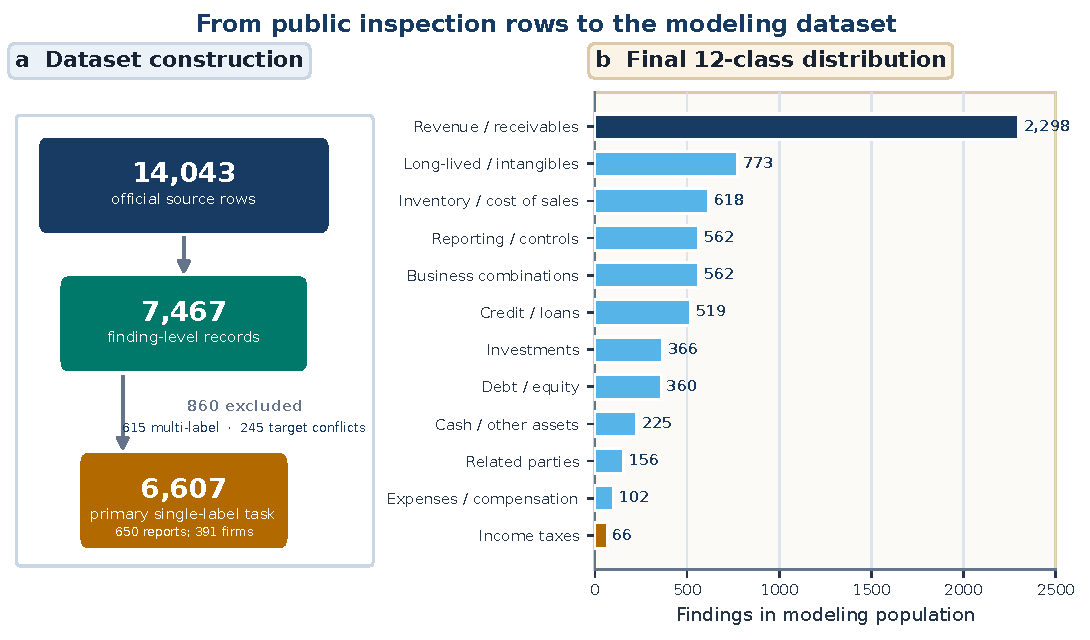
\includegraphics[width=\textwidth]{figure_assets/dataset_construction_distribution_journal_v1.pdf}%
  }{%
  \resizebox{0.98\textwidth}{!}{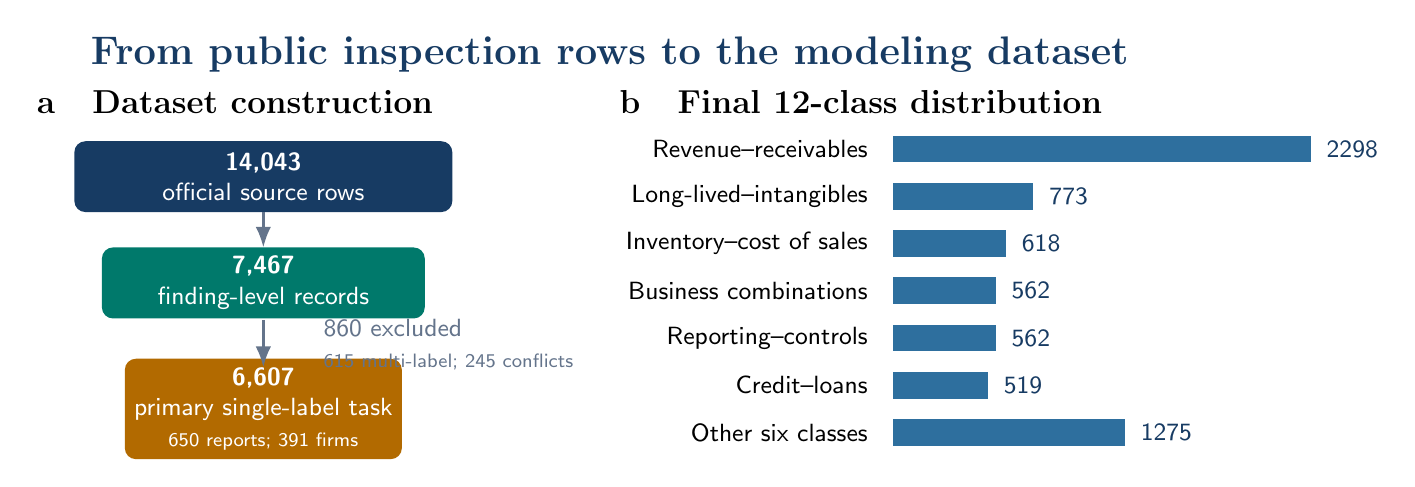
\begin{tikzpicture}[font=\sffamily\small]
    \node[font=\bfseries\Large,text=figNavy] at (7.4,5.55) {From public inspection rows to the modeling dataset};
    \node[font=\bfseries\large,anchor=west] at (0,4.95) {a\quad Dataset construction};
    \node[font=\bfseries\large,anchor=west] at (7.4,4.95) {b\quad Final 12-class distribution};
    \node[rounded corners,fill=figNavy,text=white,minimum width=4.8cm,minimum height=0.9cm,align=center] at (3.0,4.0) {\textbf{14,043}\\official source rows};
    \node[rounded corners,fill=figTeal,text=white,minimum width=4.1cm,minimum height=0.9cm,align=center] (findings) at (3.0,2.65) {\textbf{7,467}\\finding-level records};
    \node[rounded corners,fill=figAmber,text=white,minimum width=3.5cm,minimum height=1.0cm,align=center] (primary) at (3.0,1.05) {\textbf{6,607}\\primary single-label task\\\scriptsize 650 reports; 391 firms};
    \draw[-Latex,draw=figSlate,line width=1pt] (3,3.55)--(3,3.1);
    \draw[-Latex,draw=figSlate,line width=1pt] (3,2.18)--(3,1.58);
    \node[text=figSlate,align=left] at (5.35,1.87) {860 excluded\\\scriptsize 615 multi-label; 245 conflicts};
    \foreach \lab/\n/\w/\y in {Revenue--receivables/2298/5.3/4.35,Long-lived--intangibles/773/1.78/3.75,Inventory--cost of sales/618/1.43/3.15,Business combinations/562/1.30/2.55,Reporting--controls/562/1.30/1.95,Credit--loans/519/1.20/1.35,Other six classes/1275/2.94/0.75}{
      \node[anchor=east] at (10.8,\y) {\lab};
      \fill[figBlue] (11.0,{\y-0.17}) rectangle ++(\w,0.34);
      \node[anchor=west,text=figNavy] at ({11.08+\w},\y) {\n};
    }
  \end{tikzpicture}}% 
  }
  \caption{Construction and composition of the primary modeling dataset.
  \textbf{(a)} The 14,043 rows in the official source were aggregated into
  7,467 finding-level records. Excluding 615 multi-label findings and 245
  deterministic target conflicts produced the 6,607-case primary single-label
  task, spanning 650 inspection reports and 391 registered firms.
  \textbf{(b)} Counts in the final 12-class research taxonomy across all frozen
  partitions. Revenue and Receivables accounts for 2,298 findings, whereas
  Income Taxes contains 66; this imbalance motivates macro-F1, balanced
  accuracy, class weighting, and class-level diagnostics.}
  \label{fig:dataset-construction-distribution}
\end{figure*}

\begin{figure*}[t]
  \centering
  \IfFileExists{figure_assets/risk_score_comparison_journal_v1.pdf}{%
    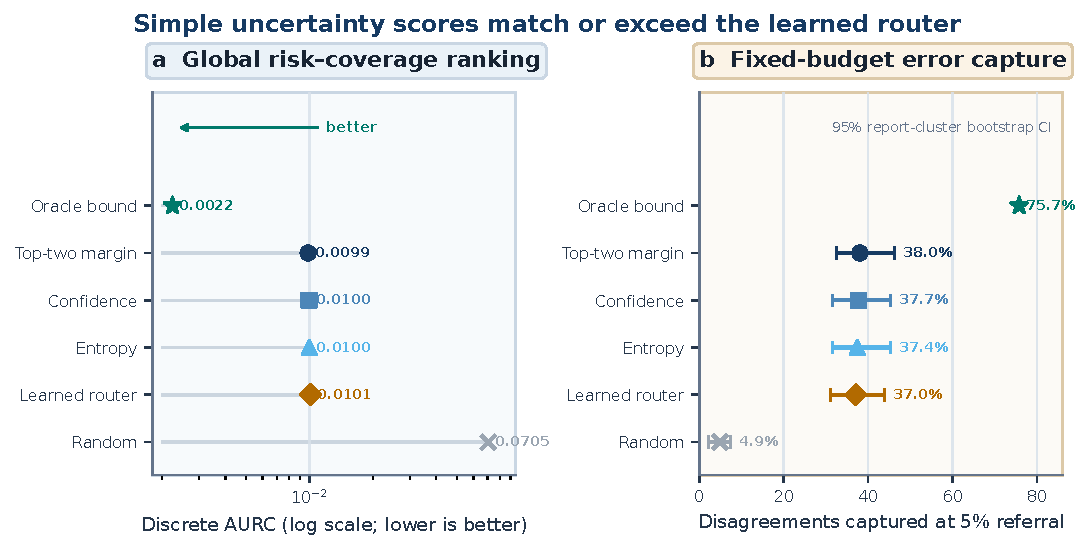
\includegraphics[width=\textwidth]{figure_assets/risk_score_comparison_journal_v1.pdf}%
  }{%
  \resizebox{0.98\textwidth}{!}{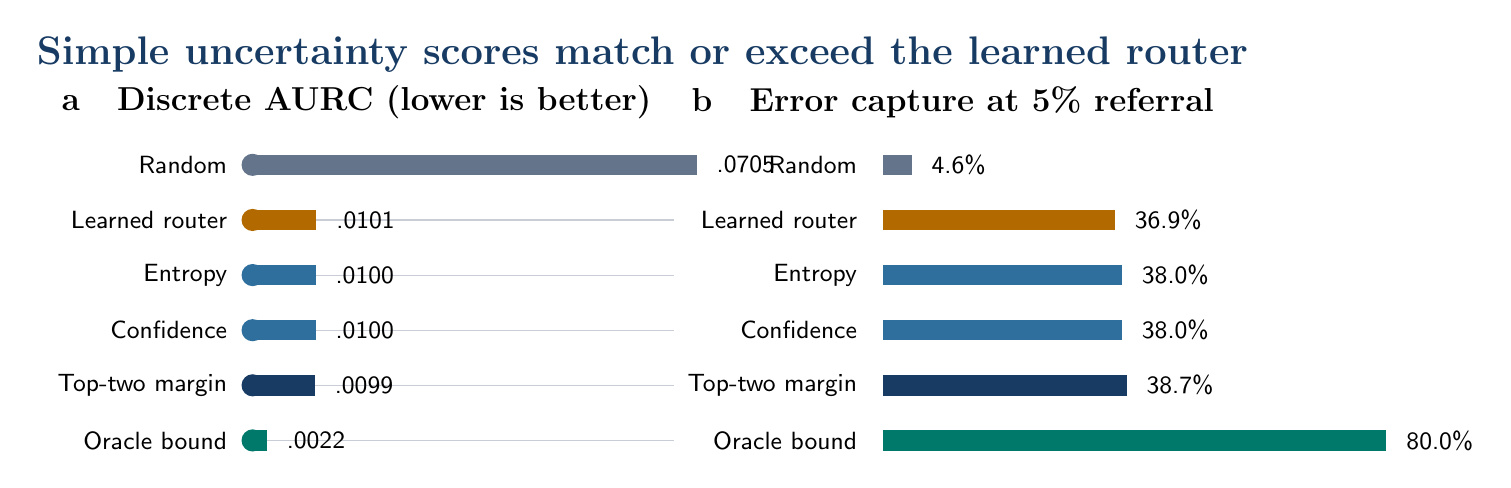
\begin{tikzpicture}[font=\sffamily\small]
    \node[font=\bfseries\Large,text=figNavy] at (7.5,5.55) {Simple uncertainty scores match or exceed the learned router};
    \node[font=\bfseries\large,anchor=west] at (0,4.95) {a\quad Discrete AURC (lower is better)};
    \node[font=\bfseries\large,anchor=west] at (8.0,4.95) {b\quad Error capture at 5\% referral};
    \foreach \lab/\v/\w/\y/\c in {Random/.0705/5.64/4.15/figSlate,Learned router/.0101/.81/3.45/figAmber,Entropy/.0100/.80/2.75/figBlue,Confidence/.0100/.80/2.05/figBlue,Top-two margin/.0099/.79/1.35/figNavy,Oracle bound/.0022/.18/.65/figTeal}{
      \node[anchor=east] at (2.35,\y) {\lab}; \draw[figSlate!35] (2.55,\y)--(7.9,\y); \fill[\c] (2.55,\y) circle (4pt); \fill[\c] (2.55,{\y-0.13}) rectangle ++(\w,0.26); \node[anchor=west] at ({2.68+\w},\y) {\v};
    }
    \foreach \lab/\v/\w/\y/\c in {Random/4.6/0.37/4.15/figSlate,Learned router/36.9/2.95/3.45/figAmber,Entropy/38.0/3.04/2.75/figBlue,Confidence/38.0/3.04/2.05/figBlue,Top-two margin/38.7/3.10/1.35/figNavy,Oracle bound/80.0/6.40/.65/figTeal}{
      \node[anchor=east] at (10.35,\y) {\lab}; \fill[\c] (10.55,{\y-0.13}) rectangle ++(\w,0.26); \node[anchor=west] at ({10.68+\w},\y) {\v\%};
    }
  \end{tikzpicture}}%
  }
  \caption{Comparison of risk-ranking scores on 4,613 clean, report-grouped
  development out-of-fold predictions. \textbf{(a)} Discrete area under the
  risk--coverage curve (AURC; lower is better) summarizes global ranking
  quality on a logarithmic scale. \textbf{(b)} Percentage of all label
  disagreements captured under a fixed 5\% referral budget; error bars denote
  95\% report-cluster bootstrap intervals. The oracle is non-deployable and is
  shown only as an attainable upper reference. Top-two margin was the best
  deployable score on both summaries, although its advantage over confidence,
  entropy, and the learned router was small.}
  \label{fig:risk-score-comparison}
\end{figure*}

\begin{figure*}[t]
  \centering
  \IfFileExists{figure_assets/class_referral_allocation_journal_v3.pdf}{%
    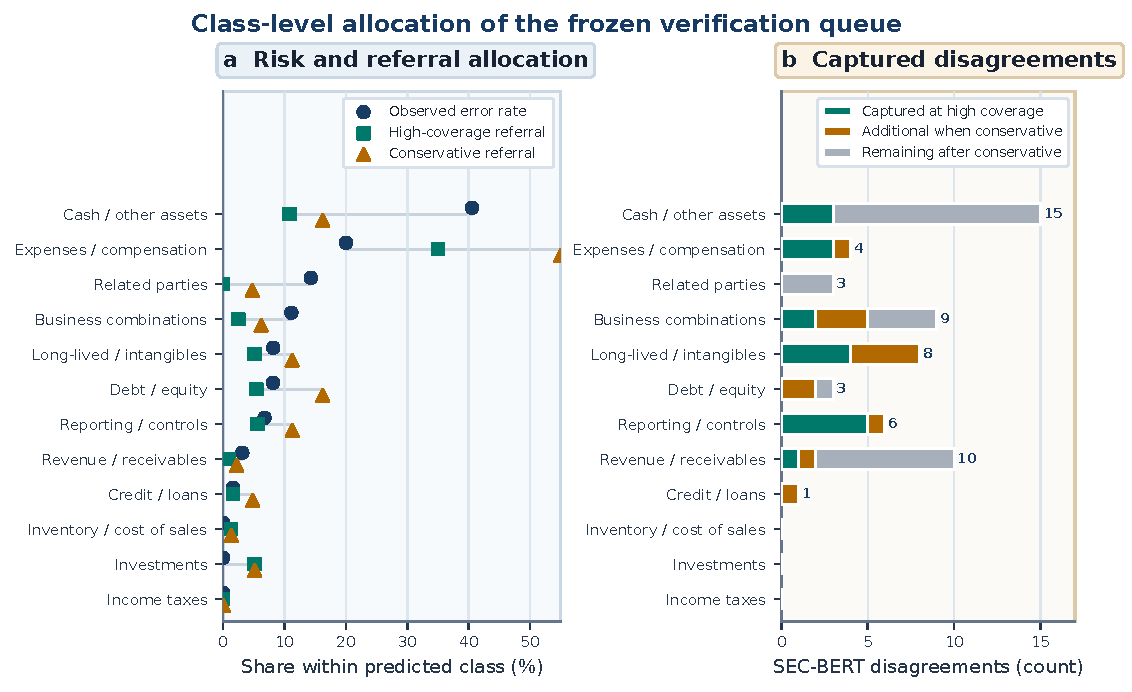
\includegraphics[width=\textwidth]{figure_assets/class_referral_allocation_journal_v3.pdf}%
  }{%
  \resizebox{0.98\textwidth}{!}{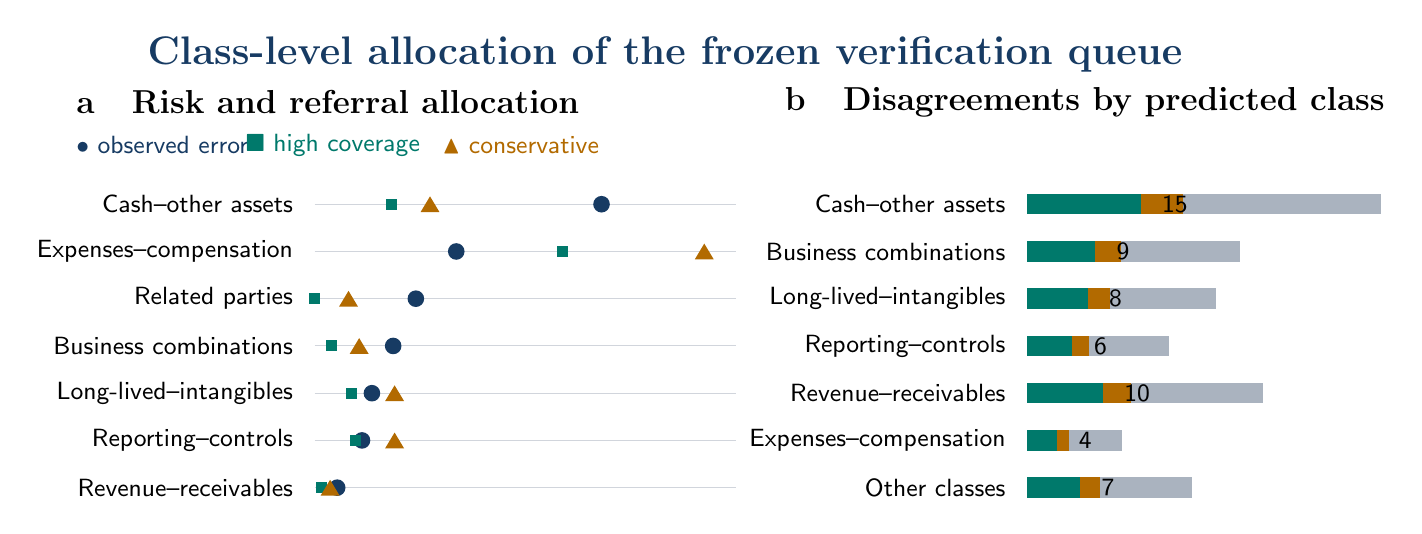
\begin{tikzpicture}[font=\sffamily\small]
    \node[font=\bfseries\Large,text=figNavy] at (7.6,5.7) {Class-level allocation of the frozen verification queue};
    \node[font=\bfseries\large,anchor=west] at (0,5.1) {a\quad Risk and referral allocation};
    \node[font=\bfseries\large,anchor=west] at (9.0,5.1) {b\quad Disagreements by predicted class};
    \node[anchor=west,text=figNavy] at (0,4.55) {$\bullet$ observed error}; \node[anchor=west,text=figTeal] at (2.15,4.55) {$\blacksquare$ high coverage}; \node[anchor=west,text=figAmber] at (4.65,4.55) {$\blacktriangle$ conservative};
    \foreach \lab/\err/\hi/\con/\y in {Cash--other assets/40.5/10.9/16.3/3.8,Expenses--compensation/20.0/35.0/55.0/3.2,Related parties/14.3/0.0/4.8/2.6,Business combinations/11.1/2.4/6.3/2.0,Long-lived--intangibles/8.1/5.2/11.3/1.4,Reporting--controls/6.7/5.8/11.3/.8,Revenue--receivables/3.2/1.0/2.2/.2}{
      \node[anchor=east] at (3.0,\y) {\lab}; \draw[figSlate!30] (3.15,\y)--(8.5,\y); \fill[figNavy] ({3.15+0.09*\err},\y) circle (3pt); \fill[figTeal] ({3.15+0.09*\hi-0.07},{\y-0.07}) rectangle ++(.14,.14); \fill[figAmber] ({3.15+0.09*\con},{\y+0.10})--++(.12,-.20)--++(-.24,0)--cycle;
    }
    \foreach \lab/\n/\w/\y in {Cash--other assets/15/4.5/3.8,Business combinations/9/2.7/3.2,Long-lived--intangibles/8/2.4/2.6,Reporting--controls/6/1.8/2.0,Revenue--receivables/10/3.0/1.4,Expenses--compensation/4/1.2/.8,Other classes/7/2.1/.2}{
      \node[anchor=east] at (12.05,\y) {\lab}; \fill[figTeal] (12.2,{\y-.13}) rectangle ++({.32*\w},.26); \fill[figAmber] ({12.2+.32*\w},{\y-.13}) rectangle ++({.12*\w},.26); \fill[figSlate!55] ({12.2+.44*\w},{\y-.13}) rectangle ++({.56*\w},.26); \node[anchor=west] at ({12.35+.32*\w},\y) {\n};
    }
  \end{tikzpicture}}%
  }
  \caption{Class-level allocation of the frozen verification queue on the
  retrospective test. Classes are defined by the SEC-BERT prediction, because
  that is the information available when a routing decision is made.
  \textbf{(a)} Observed disagreement rate and within-class referral rates under
  the frozen high-coverage and conservative policies. \textbf{(b)} SEC-BERT disagreements
  captured by the high-coverage policy, additional disagreements captured when moving
  to the conservative policy, and disagreements remaining in the automatically
  accepted set. Zero-error classes can nevertheless receive referrals because
  the global margin threshold is class-agnostic. Several classes contain few
  findings or disagreements, so these class-level allocations are descriptive
  rather than stable estimates of class-specific risk.}
  \label{fig:class-referral-allocation}
\end{figure*}

\begin{figure*}[t]
  \centering
  \IfFileExists{figure_assets/class_context_error_analysis_journal_v3.pdf}{%
    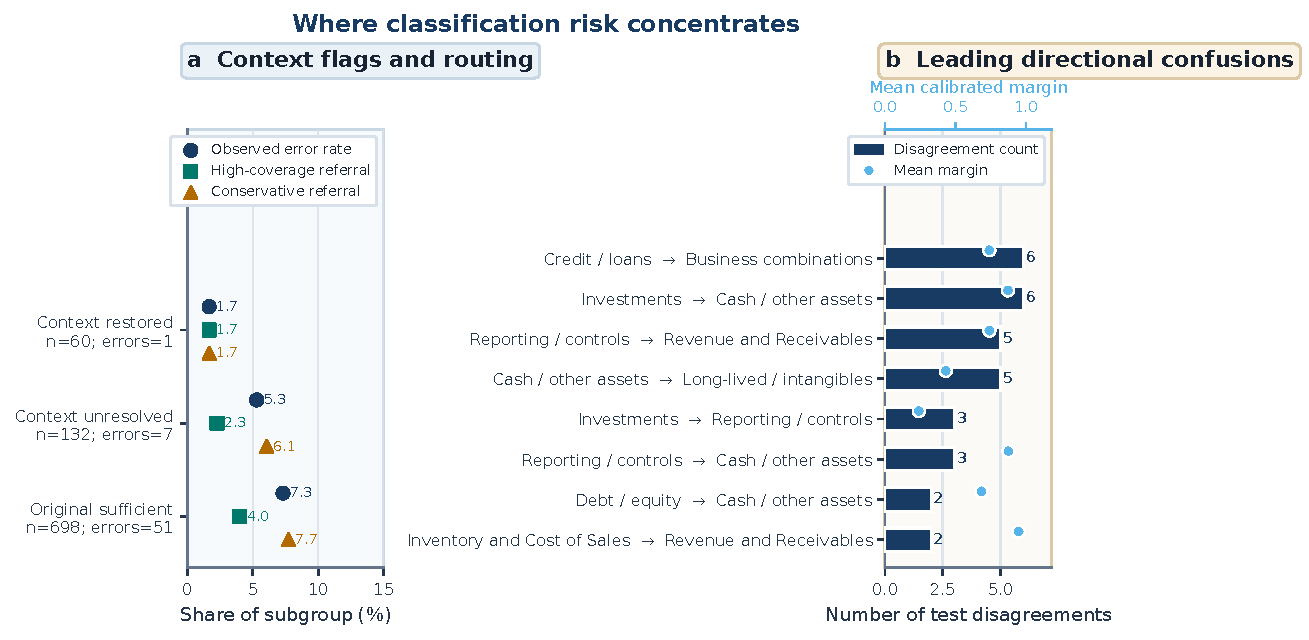
\includegraphics[width=\textwidth]{figure_assets/class_context_error_analysis_journal_v3.pdf}%
  }{%
  \resizebox{0.98\textwidth}{!}{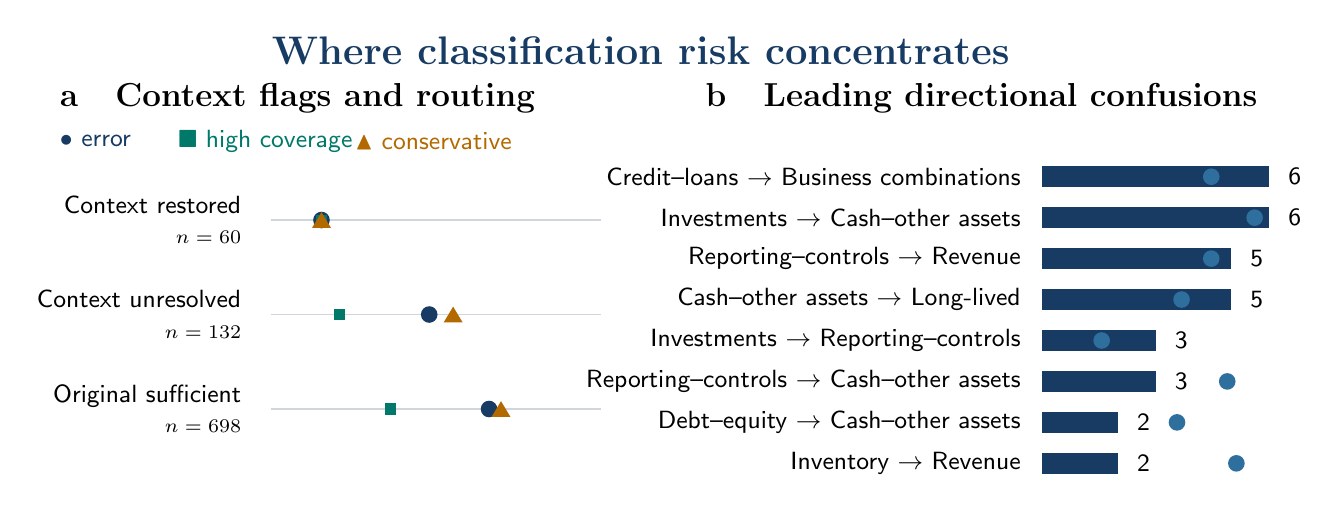
\begin{tikzpicture}[font=\sffamily\small]
    \node[font=\bfseries\Large,text=figNavy] at (7.5,5.6) {Where classification risk concentrates};
    \node[font=\bfseries\large,anchor=west] at (0,5.0) {a\quad Context flags and routing};
    \node[font=\bfseries\large,anchor=west] at (8.2,5.0) {b\quad Leading directional confusions};
    \node[anchor=west,text=figNavy] at (0,4.45) {$\bullet$ error}; \node[anchor=west,text=figTeal] at (1.5,4.45) {$\blacksquare$ high coverage}; \node[anchor=west,text=figAmber] at (3.75,4.45) {$\blacktriangle$ conservative};
    \foreach \lab/\n/\e/\h/\c/\y in {Context restored/60/1.7/1.7/1.7/3.45,Context unresolved/132/5.3/2.3/6.1/2.25,Original sufficient/698/7.3/4.0/7.7/1.05}{
      \node[anchor=east,align=right] at (2.55,\y) {\lab\\\scriptsize $n=\n$}; \draw[figSlate!30] (2.8,\y)--(7.0,\y); \fill[figNavy] ({2.8+.38*\e},\y) circle (3pt); \fill[figTeal] ({2.73+.38*\h},{\y-.07}) rectangle ++(.14,.14); \fill[figAmber] ({2.8+.38*\c},{\y+.10})--++(.12,-.20)--++(-.24,0)--cycle;
    }
    \foreach \lab/\n/\m/\y in {Credit--loans $\rightarrow$ Business combinations/6/.74/4.0,Investments $\rightarrow$ Cash--other assets/6/.93/3.48,Reporting--controls $\rightarrow$ Revenue/5/.74/2.96,Cash--other assets $\rightarrow$ Long-lived/5/.61/2.44,Investments $\rightarrow$ Reporting--controls/3/.26/1.92,Reporting--controls $\rightarrow$ Cash--other assets/3/.81/1.40,Debt--equity $\rightarrow$ Cash--other assets/2/.59/.88,Inventory $\rightarrow$ Revenue/2/.85/.36}{
      \node[anchor=east] at (12.45,\y) {\lab}; \fill[figNavy] (12.6,{\y-.13}) rectangle ++({.48*\n},.26); \fill[figBlue] ({12.6+2.9*\m},\y) circle (3pt); \node[anchor=west] at ({12.72+.48*\n},\y) {\n};
    }
  \end{tikzpicture}}%
  }
  \caption{Where SEC-BERT disagreement risk concentrates on the 890-case
  retrospective test. \textbf{(a)} Observed disagreement rate and the shares
  referred by the frozen high-coverage and conservative policies within each deterministic
  context subgroup. Counts show subgroup size and total SEC-BERT disagreements.
  The context-restored subgroup contains only one disagreement; its percentages
  should therefore be read descriptively. \textbf{(b)} The eight most frequent
  directional confusions. Bars show disagreement counts, while circles show the
  mean calibrated top-two probability margin for each confusion pair. A high
  margin denotes confident separation between the predicted class and its
  runner-up, not evidence that the PCAOB-derived target is incorrect.}
  \label{fig:class-context-errors}
\end{figure*}

\begin{figure*}[t]
  \centering
  \IfFileExists{figure_assets/sec_bert_class_performance_journal_v3.pdf}{%
    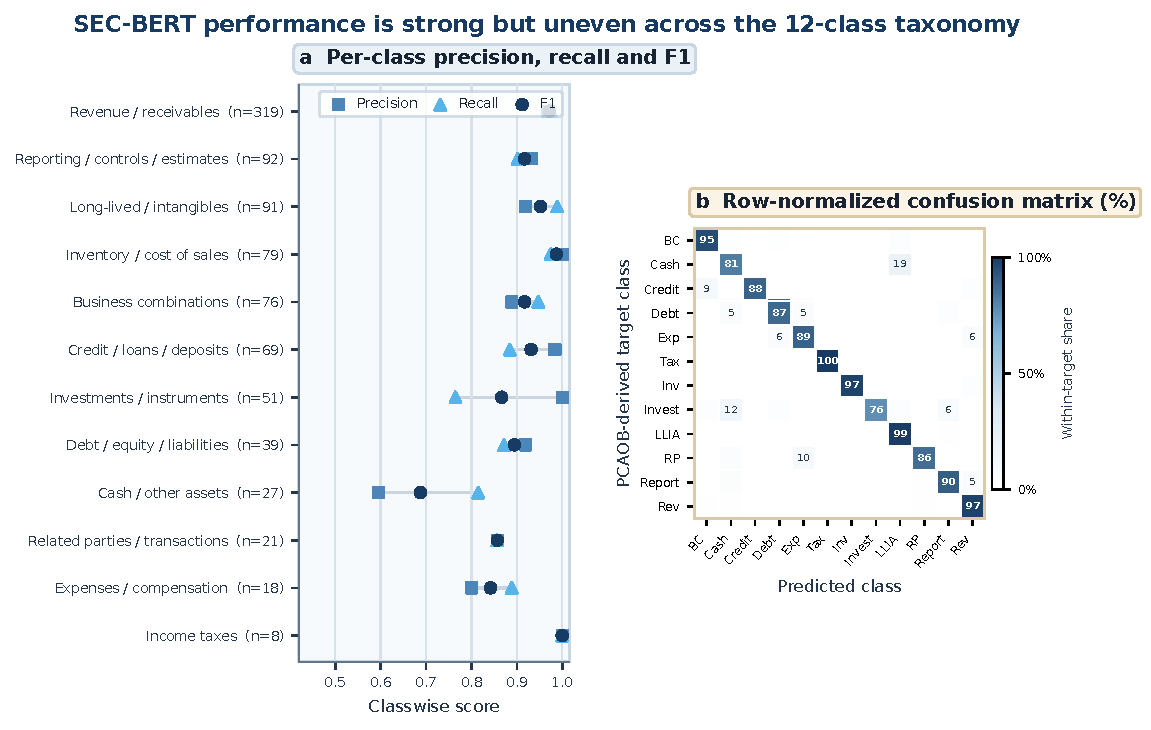
\includegraphics[width=\textwidth]{figure_assets/sec_bert_class_performance_journal_v3.pdf}%
  }{%
  \resizebox{0.98\textwidth}{!}{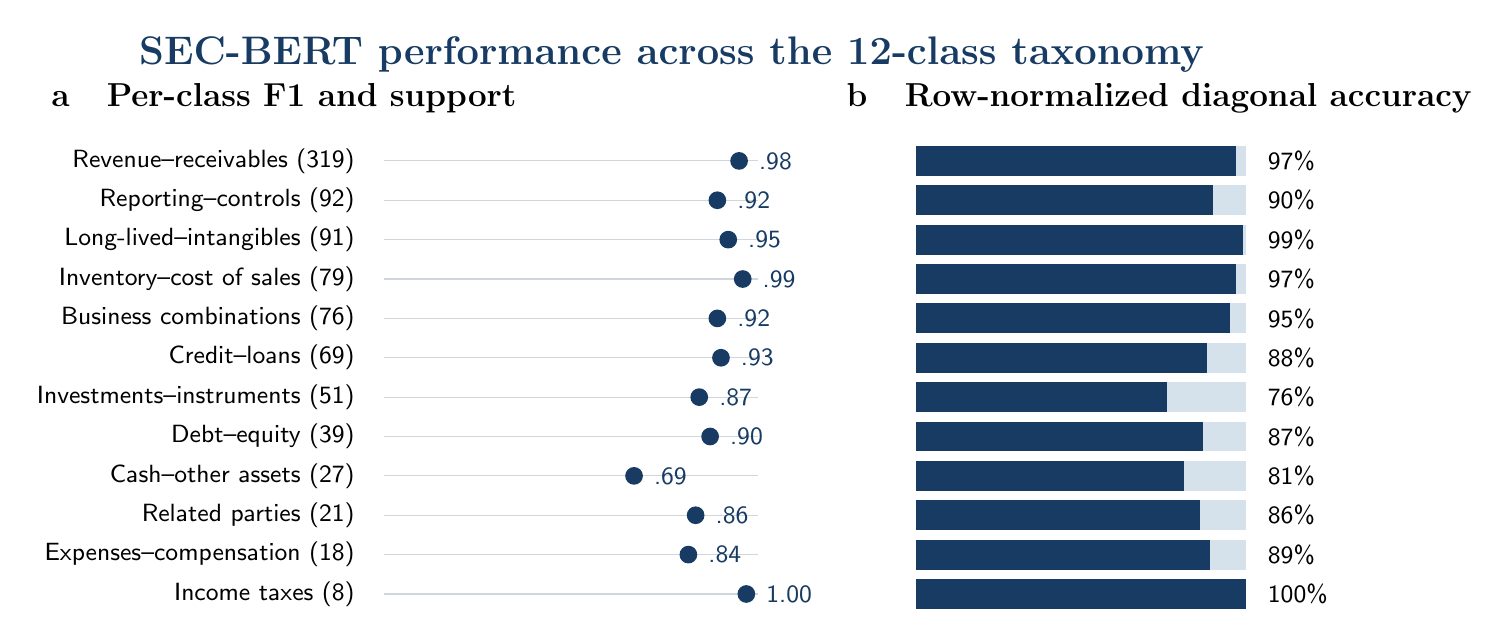
\begin{tikzpicture}[font=\sffamily\small]
    \node[font=\bfseries\Large,text=figNavy] at (8.0,7.2) {SEC-BERT performance across the 12-class taxonomy};
    \node[font=\bfseries\large,anchor=west] at (0,6.65) {a\quad Per-class F1 and support};
    \node[font=\bfseries\large,anchor=west] at (10.1,6.65) {b\quad Row-normalized diagonal accuracy};
    \foreach \lab/\n/\f/\d/\y in {Revenue--receivables/319/.98/97/5.85,Reporting--controls/92/.92/90/5.35,Long-lived--intangibles/91/.95/99/4.85,Inventory--cost of sales/79/.99/97/4.35,Business combinations/76/.92/95/3.85,Credit--loans/69/.93/88/3.35,Investments--instruments/51/.87/76/2.85,Debt--equity/39/.90/87/2.35,Cash--other assets/27/.69/81/1.85,Related parties/21/.86/86/1.35,Expenses--compensation/18/.84/89/.85,Income taxes/8/1.00/100/.35}{
      \node[anchor=east] at (4.1,\y) {\lab\ (\n)}; \draw[figSlate!30] (4.35,\y)--(9.1,\y); \fill[figNavy] ({4.35+4.6*\f},\y) circle (3.2pt); \node[anchor=west,text=figNavy] at ({4.48+4.6*\f},\y) {\f};
      \fill[figBlue!20] (11.1,{\y-.19}) rectangle ++(4.2,.38); \fill[figNavy] (11.1,{\y-.19}) rectangle ++({.042*\d},.38); \node[anchor=west] at (15.45,\y) {\d\%};
    }
  \end{tikzpicture}}%
  }
  \caption{Class-level SEC-BERT results on the 890-case clean retrospective
  test. \textbf{(a)} Precision, recall, and F1 for each class; classes are
  ordered by test support, shown in parentheses. \textbf{(b)} Confusion matrix
  normalized within each PCAOB-derived target class. Diagonal cells and
  off-diagonal cells representing at least 5\% of a target class are annotated
  as percentages. Codes are BC (Business Combinations and Consolidation), Cash
  (Cash and Other Assets), Credit (Credit, Loans, Deposits and Insurance), Debt
  (Debt, Equity and Liabilities), Exp (Expenses, Compensation and Benefits), Tax
  (Income Taxes), Inv (Inventory and Cost of Sales), Invest (Investments and
  Financial Instruments), LLIA (Long-Lived and Intangible Assets), RP (Related
  Parties and Significant Transactions), Report (Reporting, Controls, Estimates
  and Audit Procedures), and Rev (Revenue and Receivables). The estimates for
  low-support classes, especially Income Taxes ($n=8$), are descriptive.}
  \label{fig:sec-bert-class-performance}
\end{figure*}

\begin{figure*}[t]
  \centering
  \IfFileExists{figure_assets/ambiguity_signal_diagnostics_journal_v1.pdf}{%
    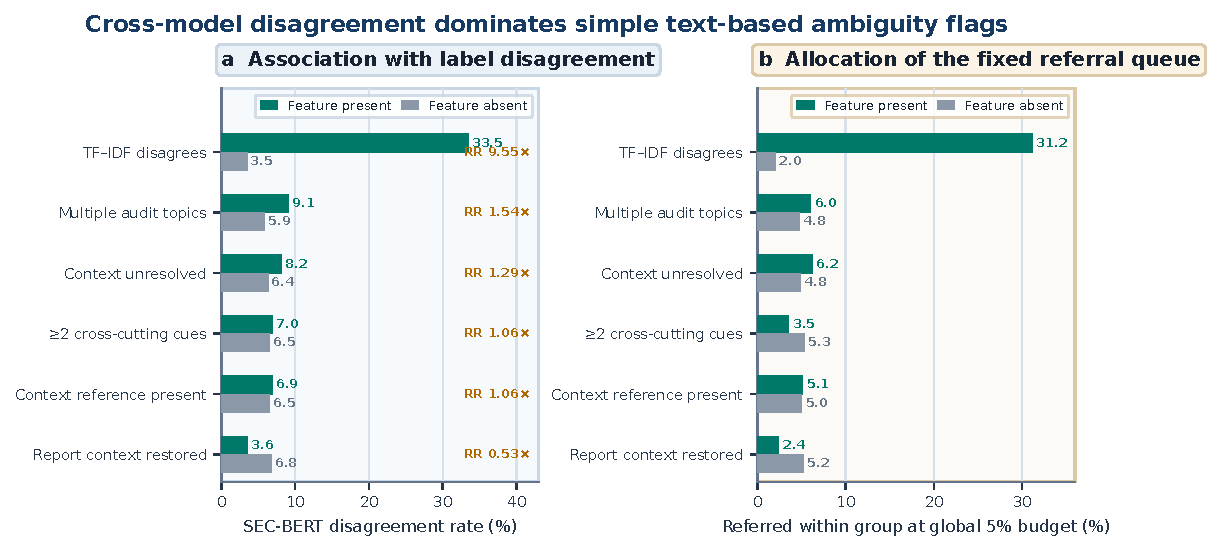
\includegraphics[width=\textwidth]{figure_assets/ambiguity_signal_diagnostics_journal_v1.pdf}%
  }{%
  \resizebox{0.98\textwidth}{!}{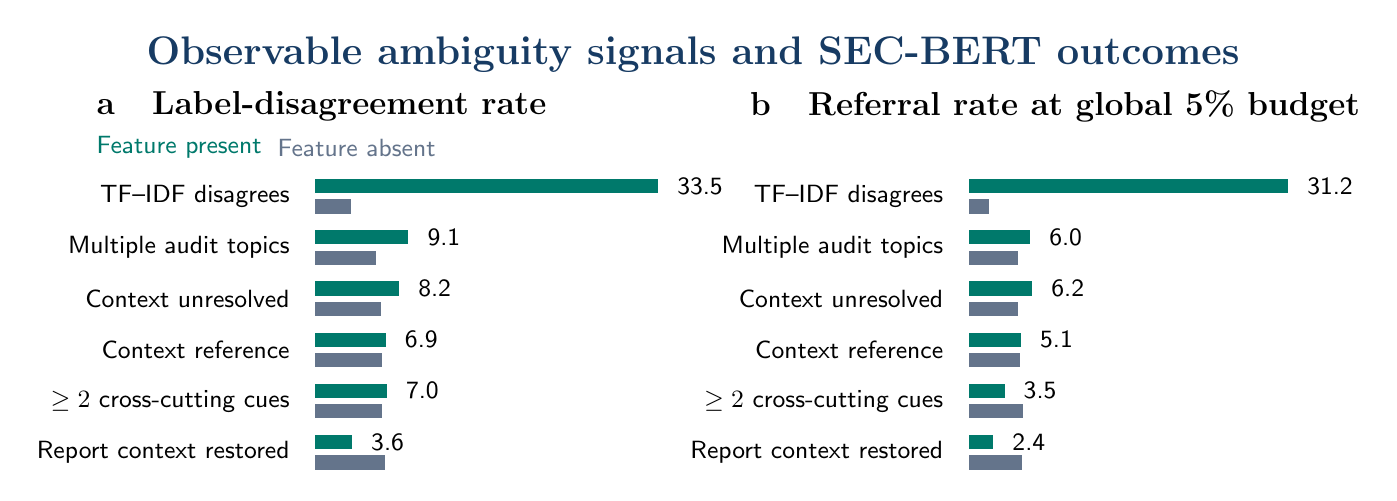
\begin{tikzpicture}[font=\sffamily\small]
    \node[font=\bfseries\Large,text=figNavy] at (7.7,5.7) {Observable ambiguity signals and SEC-BERT outcomes};
    \node[font=\bfseries\large,anchor=west] at (0,5.05) {a\quad Label-disagreement rate};
    \node[font=\bfseries\large,anchor=west] at (8.3,5.05) {b\quad Referral rate at global 5\% budget};
    \node[anchor=west,text=figTeal] at (0,4.52) {Feature present}; \node[anchor=west,text=figSlate] at (2.3,4.52) {Feature absent};
    \foreach \lab/\p/\a/\rp/\ra/\y in {TF--IDF disagrees/33.5/3.5/31.2/2.0/3.9,Multiple audit topics/9.1/5.9/6.0/4.8/3.25,Context unresolved/8.2/6.4/6.2/4.8/2.6,Context reference/6.9/6.5/5.1/5.0/1.95,$\geq2$ cross-cutting cues/7.0/6.5/3.5/5.3/1.3,Report context restored/3.6/6.8/2.4/5.2/.65}{
      \node[anchor=east] at (2.7,\y) {\lab}; \fill[figTeal] (2.9,{\y+.04}) rectangle ++({.13*\p},.18); \fill[figSlate] (2.9,{\y-.22}) rectangle ++({.13*\a},.18); \node[anchor=west] at ({3.02+.13*\p},{\y+.13}) {\p};
      \node[anchor=east] at (11.0,\y) {\lab}; \fill[figTeal] (11.2,{\y+.04}) rectangle ++({.13*\rp},.18); \fill[figSlate] (11.2,{\y-.22}) rectangle ++({.13*\ra},.18); \node[anchor=west] at ({11.32+.13*\rp},{\y+.13}) {\rp};
    }
  \end{tikzpicture}}%
  }
  \caption{Descriptive associations between observable ambiguity signals and
  SEC-BERT outcomes on 4,613 clean report-grouped development out-of-fold
  predictions. \textbf{(a)} Label-disagreement rates when each feature is
  present or absent. RR denotes the ratio of the two rates. \textbf{(b)} Share
  referred within the same groups by the globally defined 5\% top-two-margin
  policy. Feature-present sample sizes were 478 for TF--IDF disagreement, 997
  for multiple audit topics, 645 for unresolved context, 733 for at least two
  cross-cutting cues, 896 for a context reference, and 250 for restored report
  context. Features overlap and were produced by deterministic rules rather
  than expert ambiguity labels. The figure therefore demonstrates diagnostic
  association, not causation or professional adjudication.}
  \label{fig:ambiguity-signal-diagnostics}
\end{figure*}

\section{Frozen Temporal Protocol}
\label{app:temporal-protocol}

The prospective evaluation is anchored to the official PCAOB Part~I.A snapshot
archived on September 27, 2026. That file contained 14,043 parsed rows and had
SHA-256 digest
\texttt{af543784fa73475741e20324ce451b1de1df96fe4a826fd292b1f9aa4b7c96d7}.
A later snapshot becomes eligible only when its file digest differs from this
reference. Before inspecting labels or model outputs, the new source file must
be archived, hashed, and compared by the same stable report identity used in the
development protocol.

Only findings from report identities absent from the frozen snapshot enter the
temporal holdout. Expanded disclosures from an already observed report do not
qualify merely because additional sections later became public. Eligible new
reports are processed using the frozen aggregation, cleaning, context repair,
taxonomy, and near-duplicate rules. Findings that fail those rules are excluded
without modifying the rules or substituting additional cases.

The stored SEC-BERT weights are then applied without further training. The
temperature remains fixed at $1.1517754200$, the risk score remains the
calibrated top-two probability margin, and the primary and conservative
thresholds remain $0.5269052934$ and $0.8157442331$, respectively. Model,
preprocessing, threshold, eligibility, and metric choices may not be revised in
response to the new labels. The evaluation reports full-automation accuracy and
macro-F1, coverage and selective accuracy for both policies, disagreement
capture, verification precision, class-level outcomes, and report-cluster
uncertainty when the number of new reports permits meaningful resampling.

The official file checked on October 13, 2026 was byte-identical to the frozen
snapshot and supplied zero eligible report identities. The temporal protocol is
therefore locked but unexecuted; the next refresh begins with the file-hash
comparison and stops immediately if the digest is unchanged.

\end{document}
